
\documentclass{article}
\usepackage[utf8]{inputenc}

\usepackage[table]{xcolor}
\usepackage[HTML]{xcolor}
\usepackage[utf8]{inputenc}
\usepackage[T1]{fontenc}
\usepackage{listings}
\usepackage{tabularx}
\usepackage{multirow}
\usepackage{amsmath}
\usepackage{adjustbox}
\usepackage{amssymb}
\usepackage{graphicx}
\usepackage{array}
\newcolumntype{L}[1]{>{\raggedright\arraybackslash}p{#1}}
\newcolumntype{C}[1]{>{\centering\arraybackslash}p{#1}}
\usepackage{svg}
\usepackage[margin=1in]{geometry}
\usepackage{booktabs}
\usepackage{array}
\usepackage{pdflscape}
\usepackage{blindtext}
\usepackage{tikz}
\usetikzlibrary{trees}
\usepackage{minted} 
\usepackage{fancyhdr}
\usepackage[colorlinks=true, linkcolor=gray, urlcolor=gray, citecolor=gray, filecolor=gray]{hyperref}
\usepackage{soul}
\usepackage{float}
\definecolor{primary}{RGB}{43, 108, 176}
\definecolor{codebg}{RGB}{247, 250, 252}
\definecolor{jsonkey}{RGB}{197, 48, 48}
\definecolor{jsonstring}{RGB}{44, 122, 123}
\definecolor{jsonnumber}{RGB}{116, 44, 122}

\lstdefinelanguage{json}{
    basicstyle=\small\ttfamily,
    backgroundcolor=\color{codebg},
    stringstyle=\color{jsonstring},
    keywordstyle=\color{jsonkey}\bfseries,
    commentstyle=\color{gray},
    numbers=none,
    breaklines=true,
    showstringspaces=false
}

% Custom commands (from D2)
\newcommand{\obsub}[1]{%
  \stepcounter{OBnum}%
  \addcontentsline{toc}{subsubsection}{OB \arabic{OBnum} - #1}%
  \subsection*{OB \arabic{OBnum} - #1}%
}
\newcounter{OBnum}

% Header and footer
\pagestyle{fancy}
\fancyhf{} 
\setlength{\headheight}{20pt}
\fancyhead[R]{104 - Team Not Found \\ version 1.0}
\fancyfoot[C]{\thepage}
\renewcommand{\headrulewidth}{0.4pt}

\begin{document}
\clearpage
\thispagestyle{empty}
\hbox{}
\clearpage
% --- TITLE PAGE ---
\begin{titlepage}

    \centering 
    {\Huge\bfseries Implementation of the software \par}
    \vspace{0.5cm}
    {\Large\itshape from design to working prototype\par}
    \vspace{2cm}
    
    \begin{figure}[h]
        \centering
        
\includegraphics[width=1.0\textwidth]{104okok.png}
    \end{figure}
    
    \vfill

    {\Huge \textbf{104 - Team Not Found}} \\
    \vspace{0.55cm}

    \begin{flushright}
        {\large \textbf{Matteo Golinelli, Caterina Alessi, Robin Bertolini, Virginia Ancora}} \\
        \vspace{0.1cm}
        {\large \textit{\today}}
    \end{flushright}
\end{titlepage}

\cleardoublepage
\tableofcontents
\newpage

% ============================================================================
% SECTION: PURPOSE OF THE DOCUMENT
% ============================================================================
\section{Purpose of the Document}
This document synthesize. all the most important information necessary for the development of the train application of 104 (s)team not found. It includes the user flows related to 
the actions that can be performed by anonymous users, registered users and system users (ticket inspector, system admin), the document continues with the presentation of the required APIs that are both simulated and actually implemented used for example to log in, register, delete an account ecc. For each API created, in addition to a description of the features provided, the document presents its documentation. 
The information about the Git Repository and the actual application deployment are covered in the final section.

% ============================================================================
% SECTION: ARCHITECTURE CHOICE AND LANGUAGE USED
% ============================================================================
\section{Architecture Choice and Language Used}
\subsection{Architecture Type}
The architecture of the system is a client-server type based on the web, the backhand is developed with Node.js while the front-end of the web-app is in HTML/CSS/JS. The architecture is structured so that the backend exposes some API that handle the logic such as for the ticket management, train search and so on. The front-end uses API to present a user interface with different pages, some of which are accessible only with the right credentials (i.e. ticket inspector page, admin page). All the data stored in a separated databases simulated by a \texttt{.json} file. This architectural choice is motivated by the need for simplicity for development, scalability, and maintainability, leaving space for future extensions (e.g., adding new APIs or UI features).  

\subsection{Programming Language}
The web-app is implemented using JavaScript with Node.js for the back-end. The front-end uses standard web technologies (HTML/CSS/JS). The choice of Node.js is driven by its simplicity and fast prototyping feature, moreover Express along with other frameworks offers one of the best API requests handling. Additionally JavaScript blends well with the front-end  programming language choice. 

\subsection{Dependencies}
The project dependencies are defined in \texttt{package.json} that includes both library used for backend and  frontend.

\subsection*{Backend (Node.js):}
\begin{itemize}
    \item \texttt{Express}
\end{itemize}
(No other backend dependencies; all other operation uses native modules like: \texttt{fs}, \texttt{crypto}, \texttt{path}, \texttt{url}.)

\subsection*{Frontend:}
\begin{itemize}
    \item \textbf{Leaflet} (\texttt{leaflet.css} / \texttt{leaflet.js}) -- map.
    \item \textbf{QRCode.js} -- qr code generation.
    \item \textbf{html5-qrcode} -- qr code scan.
\end{itemize}
\newpage

\subsection{Database}
The database is unique and stores entries for: 
\begin{itemize}
    \item \texttt{stations}
    \item \texttt{routes}
    \item \texttt{trainRuns}
    \item \texttt{users}
    \item \texttt{tickets}
    \item \texttt{payments}
    \item \texttt{subscriptions}
\end{itemize}

\section*{Sample Schema Definitions}
Following there are some examples of principal data structures entries:
\subsection{Stations Collection Document (\texttt{stations})}
\begin{lstlisting}[language=json]
{
  "_id": "64871f2a2b13f99e0137a001",
  "stationId": 1,
  "name": "Trento",
  "city": "Trento",
  "code": "TN",
  "region": "Trentino-Alto Adige",
  "latitude": 46.0667,
  "longitude": 11.1167,
  "__v": 0
}
\end{lstlisting}

\subsection{Operational Route Document Schema (\texttt{routes})}
\begin{lstlisting}[language=json]
{
  "_id": "64871f502b13f99e0137a309",
  "routeId": 1,
  "routeName": "Ferrovia della Valsugana (Trento - Bassano)",
  "stops": [
    { "stopOrder": 1, "stationId": 1, "scheduledArrival": null, "scheduledDeparture": "06:00", "trackNumber": 2 },
    { "stopOrder": 2, "stationId": 4, "scheduledArrival": "06:40", "scheduledDeparture": "06:42", "trackNumber": 1 },
    { "stopOrder": 3, "stationId": 3, "scheduledArrival": "07:10", "scheduledDeparture": "07:12", "trackNumber": 1 },
    { "stopOrder": 4, "stationId": 5, "scheduledArrival": "07:55", "scheduledDeparture": null, "trackNumber": 3 }
  ],
}
\end{lstlisting}

\subsection{Train Run Collection Document (\texttt{trainRuns})}
\begin{lstlisting}[language=json]
{
  "_id": "64871f612b13f99e0137b412",
  "runId": 102,
  "trainId": 2,
  "routeId": 3,
  "departureDateTime": "2026-06-01T07:00:00",
  "status": "delayed",
  "currentDelayMinutes": 10,
  "actualDeparture": "2026-06-01T07:10:00",
  "actualArrival": null,
}
\end{lstlisting}

\subsection{User Collection Document (\texttt{users})}
\begin{lstlisting}[language=json]
{
  "_id": "64871f3a2b13f99e0137a101",
  "userId": 1001,
  "name": "Matteo",
  "surname": "Golinelli",
  "email": "matteo.golinelli@studenti.unitn.it",
  "passwordHash": "$2b$12$R9hKeQy7fzgD6V5gSioTaQjUY3xrG",
  "role": "passenger",
  "preferredLanguage": "it",
  "loyaltyPoints": 320,
  "failedLoginAttempts": 0,
  "accountStatus": "active",
}
\end{lstlisting}

\subsection{Ticket Document Schema (\texttt{tickets})}
\begin{lstlisting}[language=json]
{
  "_id": "64871f452b13f99e0137a204",
  "ticketId": 5001,
  "ticketCode": "TKT-1001-001",
  "userId": 1001,
  "runId": 101,
  "fromStopOrder": 1,
  "toStopOrder": 4,
  "passengerType": "adult",
  "seatNumber": "12B",
  "class": "standard",
  "price": 12.50,
  "status": "active",
  "purchaseDate": "2026-05-28T10:15:00",
  "qrCode": "QR5001ABC",
  }
\end{lstlisting}

\subsection{Transactional Payments Document (\texttt{payments})}
\begin{lstlisting}[language=json]
{
  "_id": "64871f722b13f99e0137c523",
  "paymentId": 4001,
  "userId": 1001,
  "ticketId": 5001,
  "subscriptionId": null,
  "amount": 17.50,
  "paymentDate": "2026-05-28T10:18:00",
  "paymentMethod": "Visa",
  "transactionId": "TXN1001",
  "status": "completed",
}
\end{lstlisting}

\subsection{Subscriptions Document (\texttt{subscriptions})}
\begin{lstlisting}[language=json]
{
      "subscriptionId": 2001,
      "userId": 1004,
      "fromStationId": 15,
      "toStationId": 20,
      "startDate": "2026-05-01",
      "endDate": "2026-07-31",
      "class": "standard",
      "price": 220,
      "status": "active"
}
\end{lstlisting}


% ============================================================================
% SECTION: USER FLOWS
% ============================================================================
\newpage
\section{User Flows}

\subsection{Authentication/Specific Access Flow}
- Related FR: FR12, FR28, FR34, FR31

\begin{figure}[H]
    \centering
    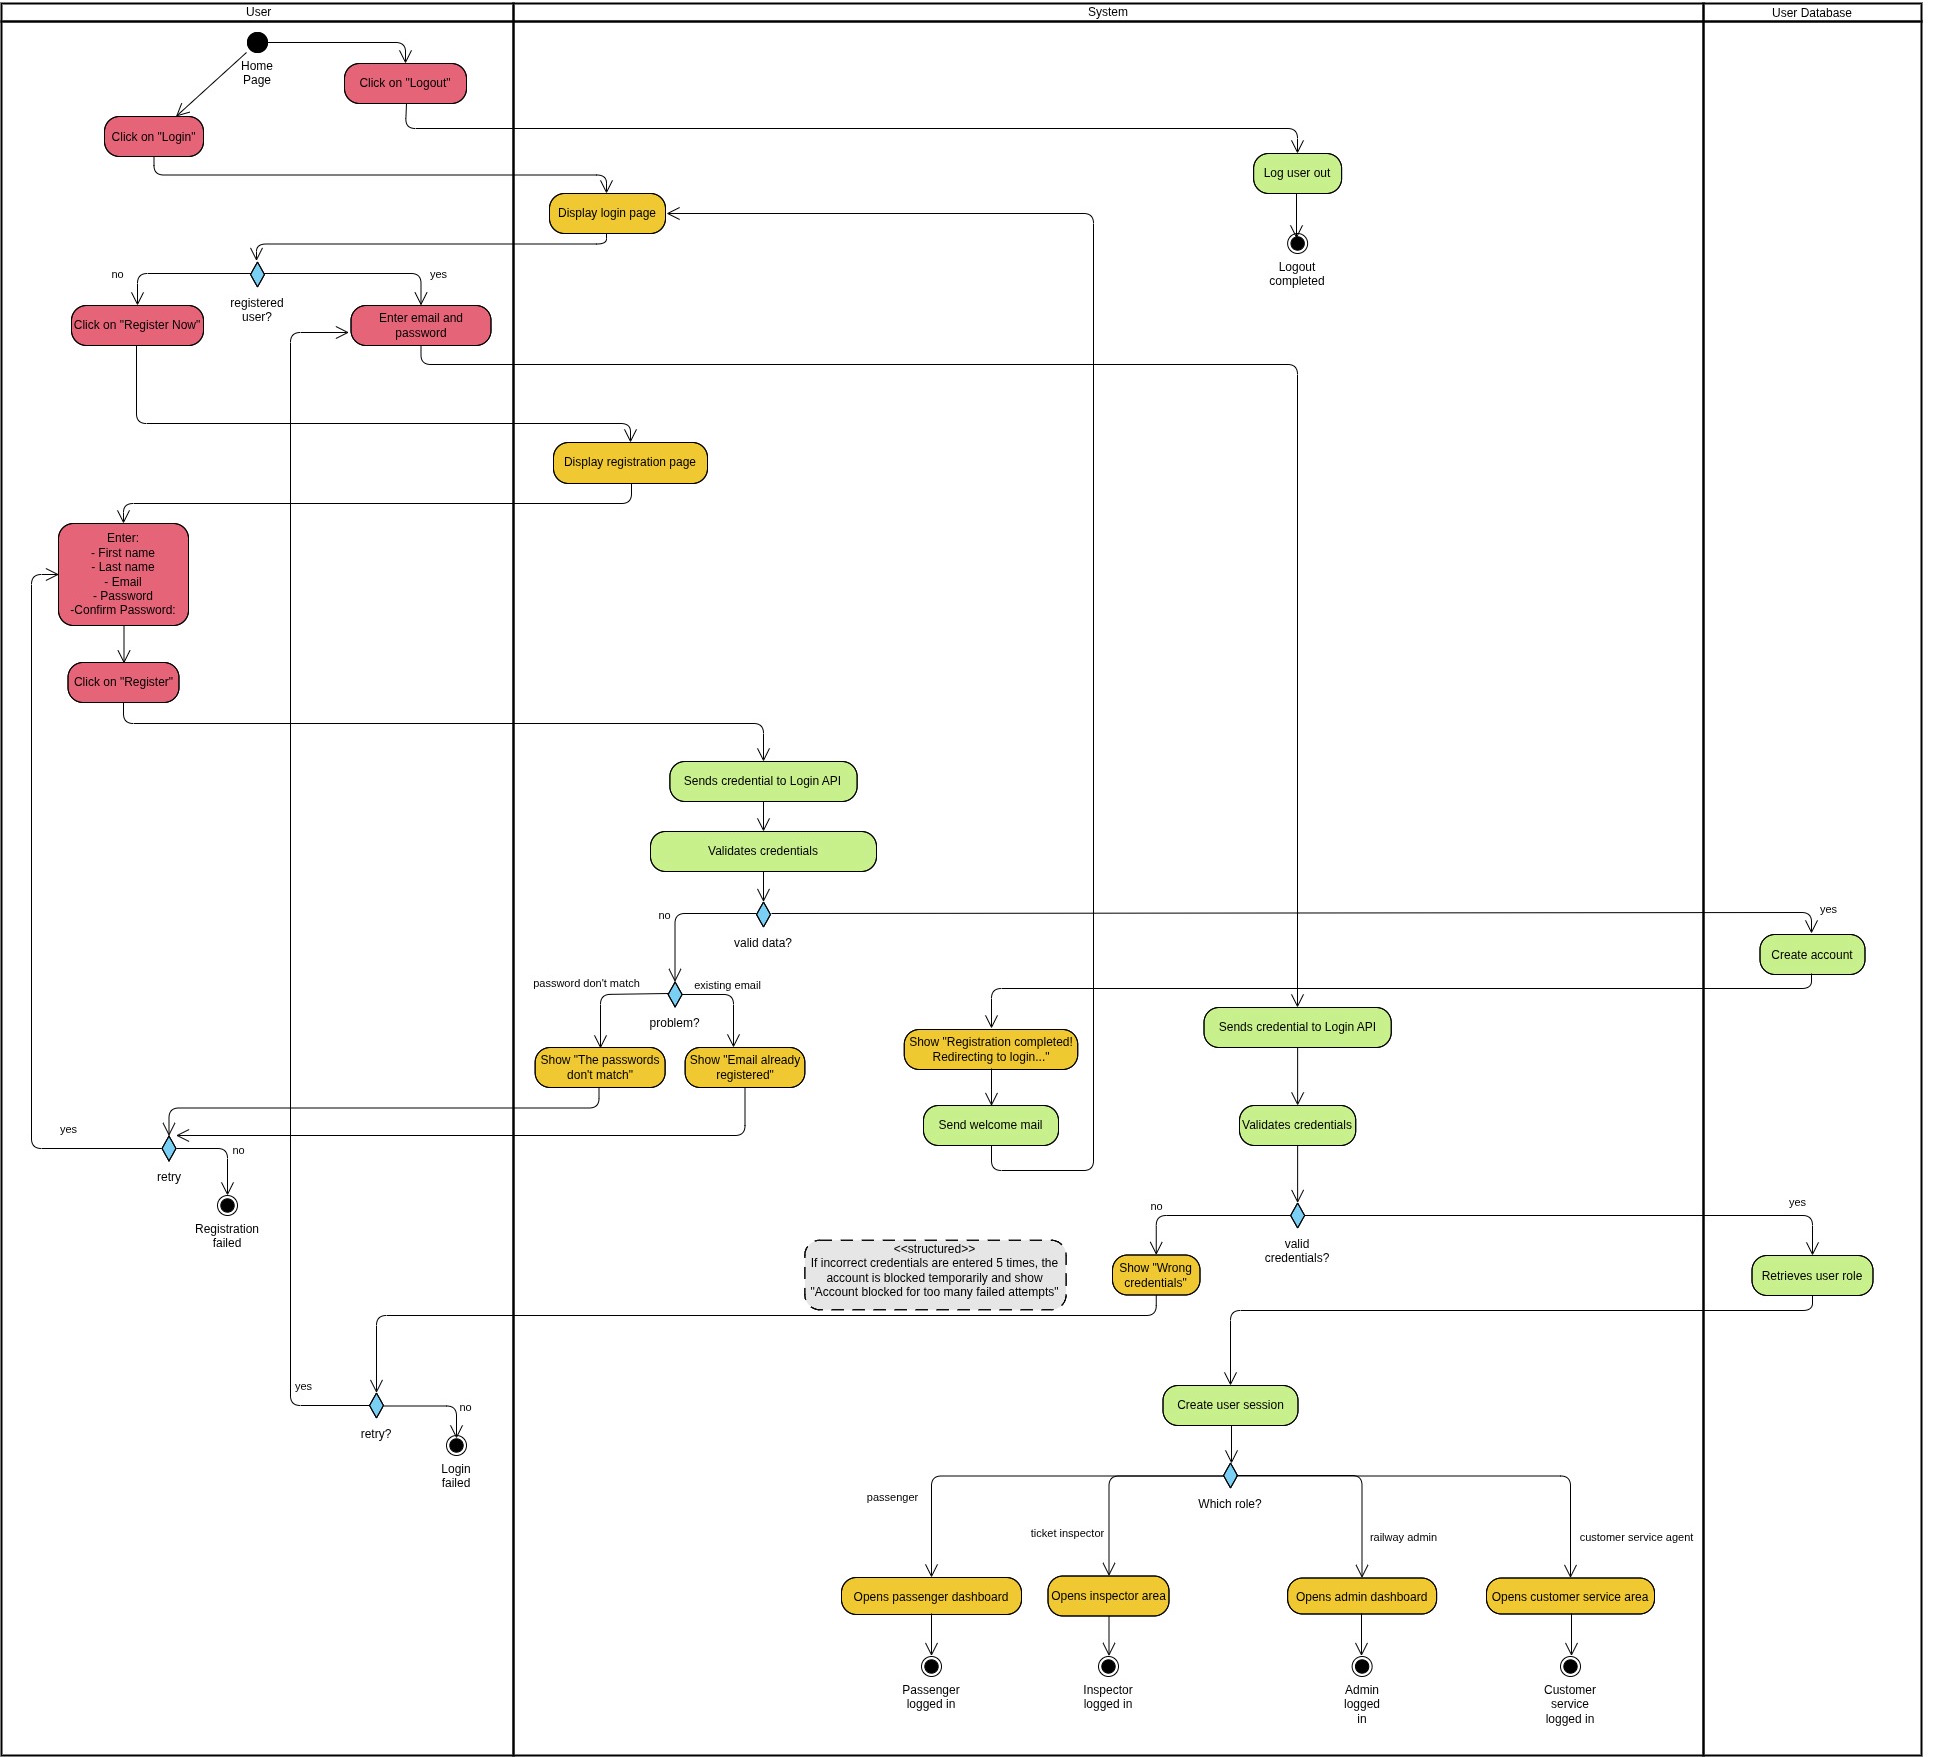
\includegraphics[width=0.9\linewidth]{Authentication_Specific Access Flow.jpg}
    \label{fig:placeholder}
\end{figure}
\newpage

\subsection{Account Management Flow}
-Related FR: FR27, FR29, FR30
\begin{figure}[H]
    \centering
    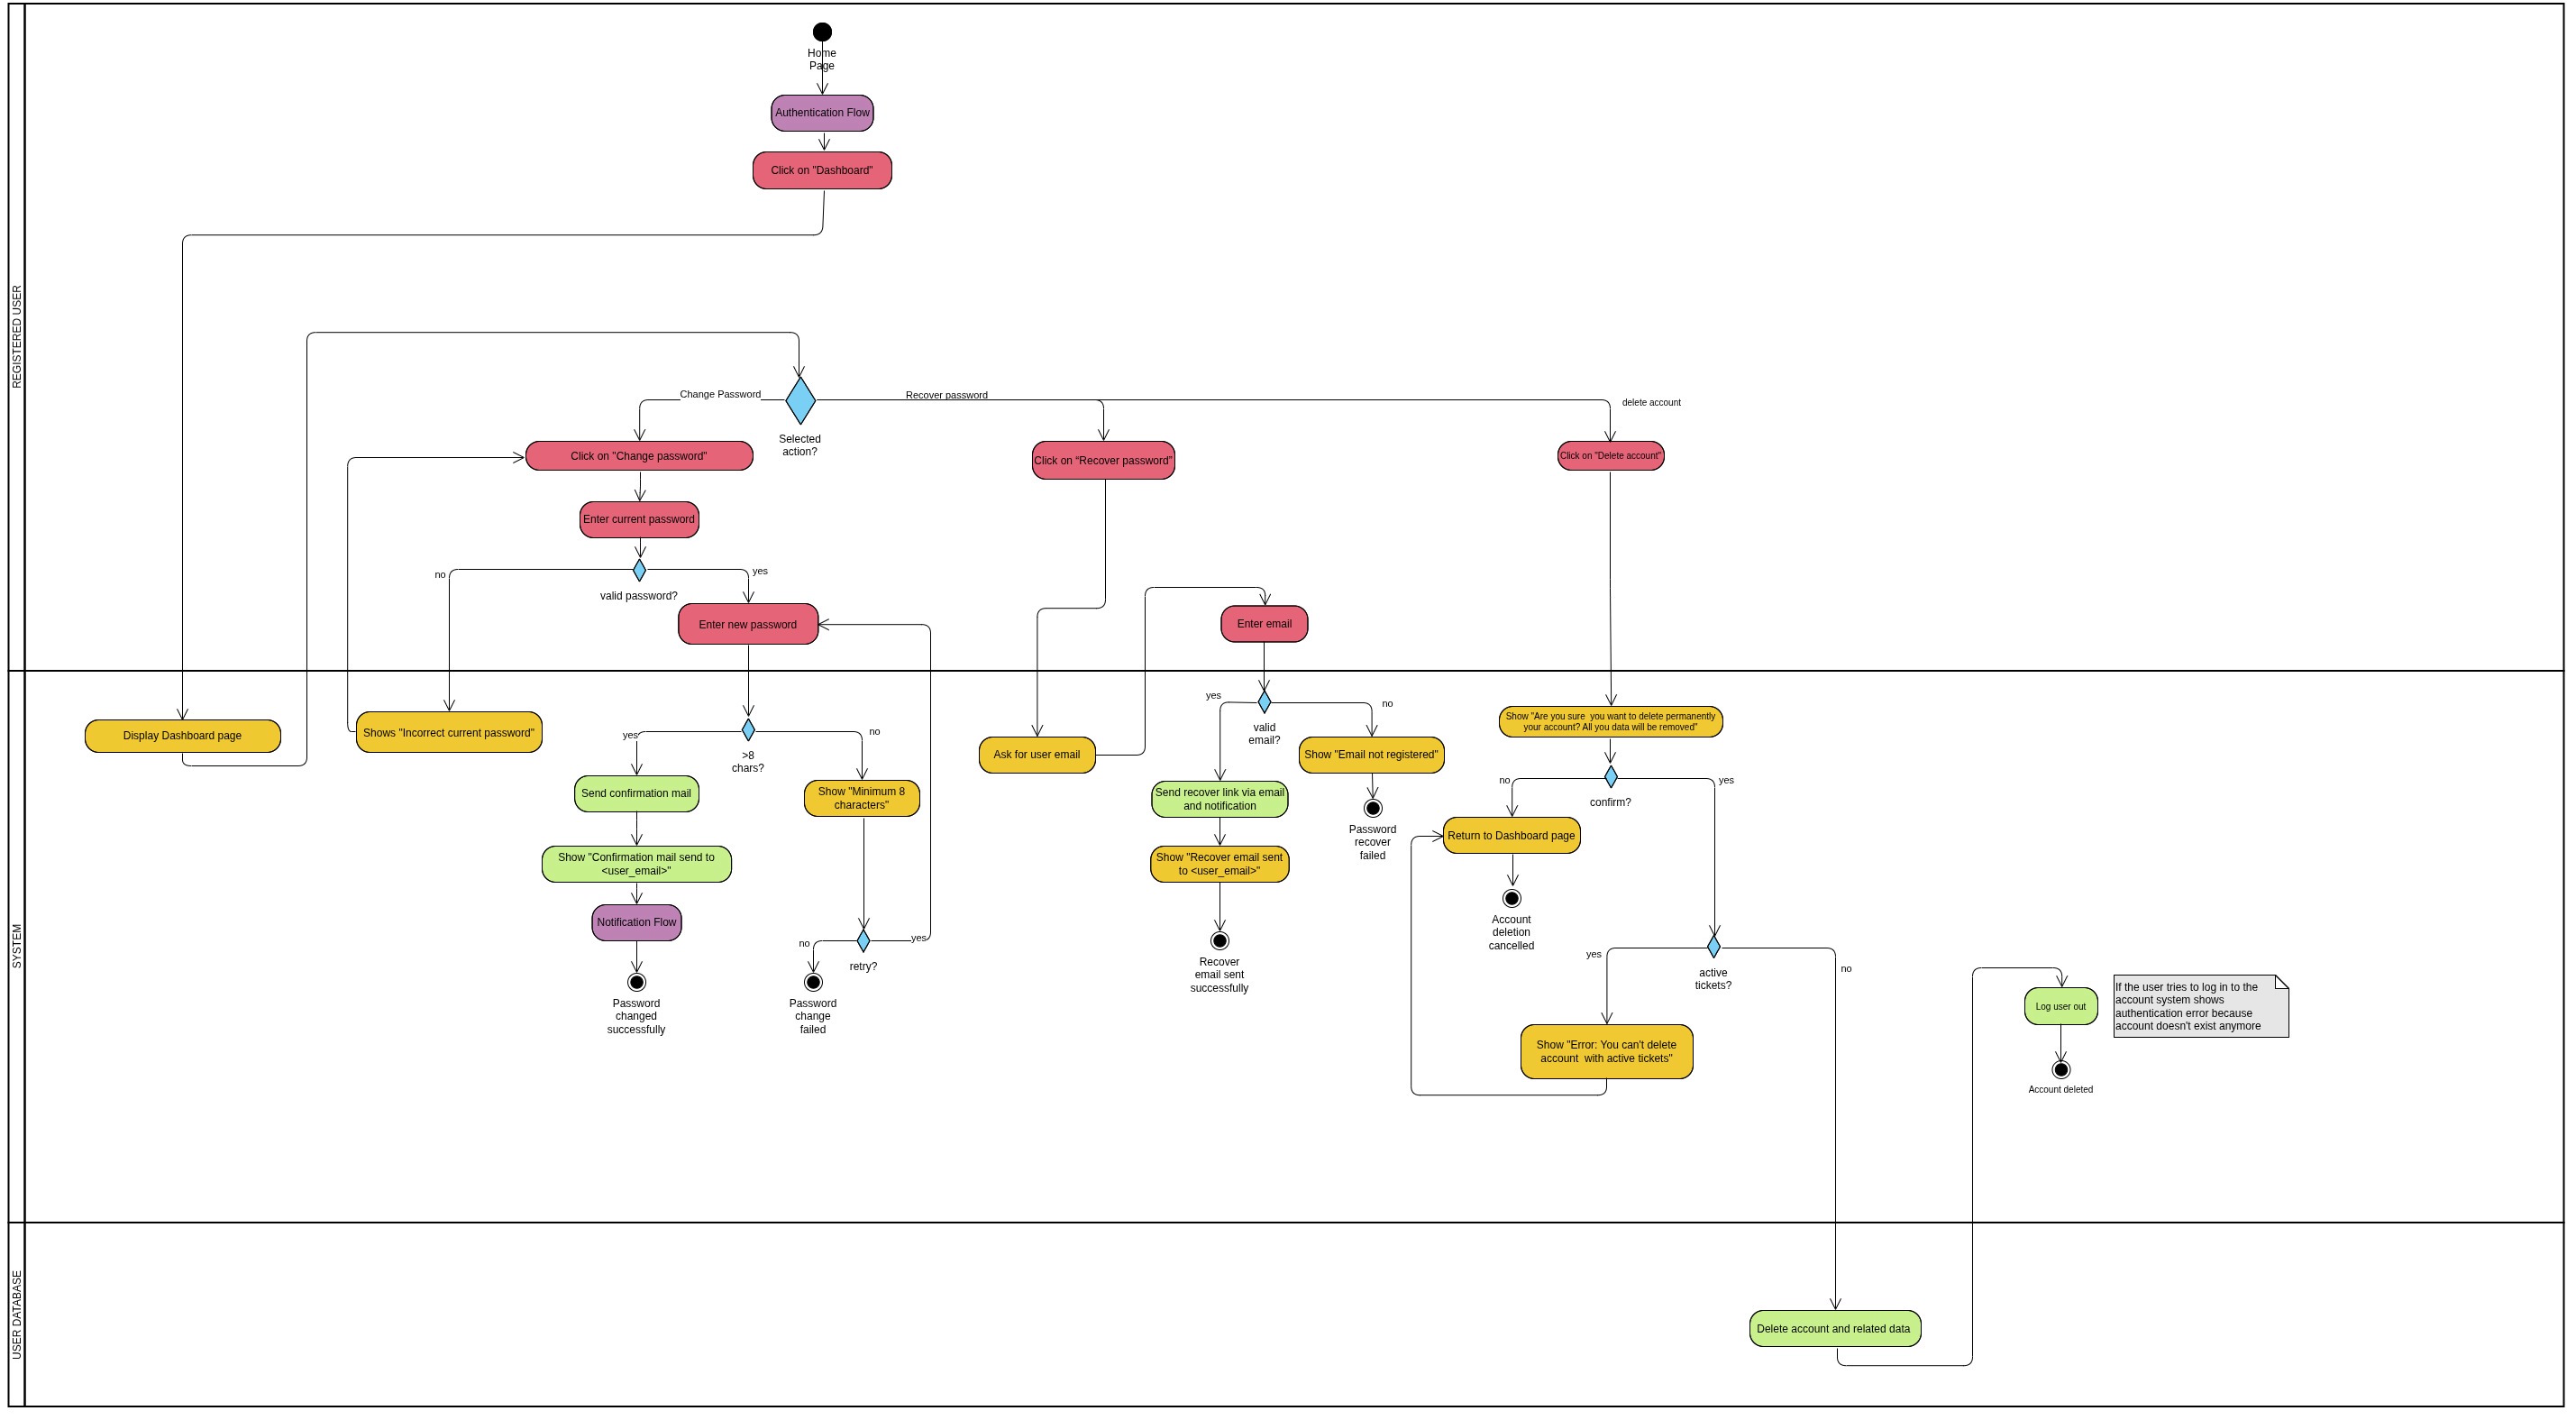
\includegraphics[width=0.9\linewidth]{Account Management Flow.jpg}
    \label{fig:placeholder}
\end{figure}
\newpage

\subsection{Train Status and Delay Prediction Flow}
-Related FR: FR5, FR15, FR33
\begin{figure}[H]
    \centering
    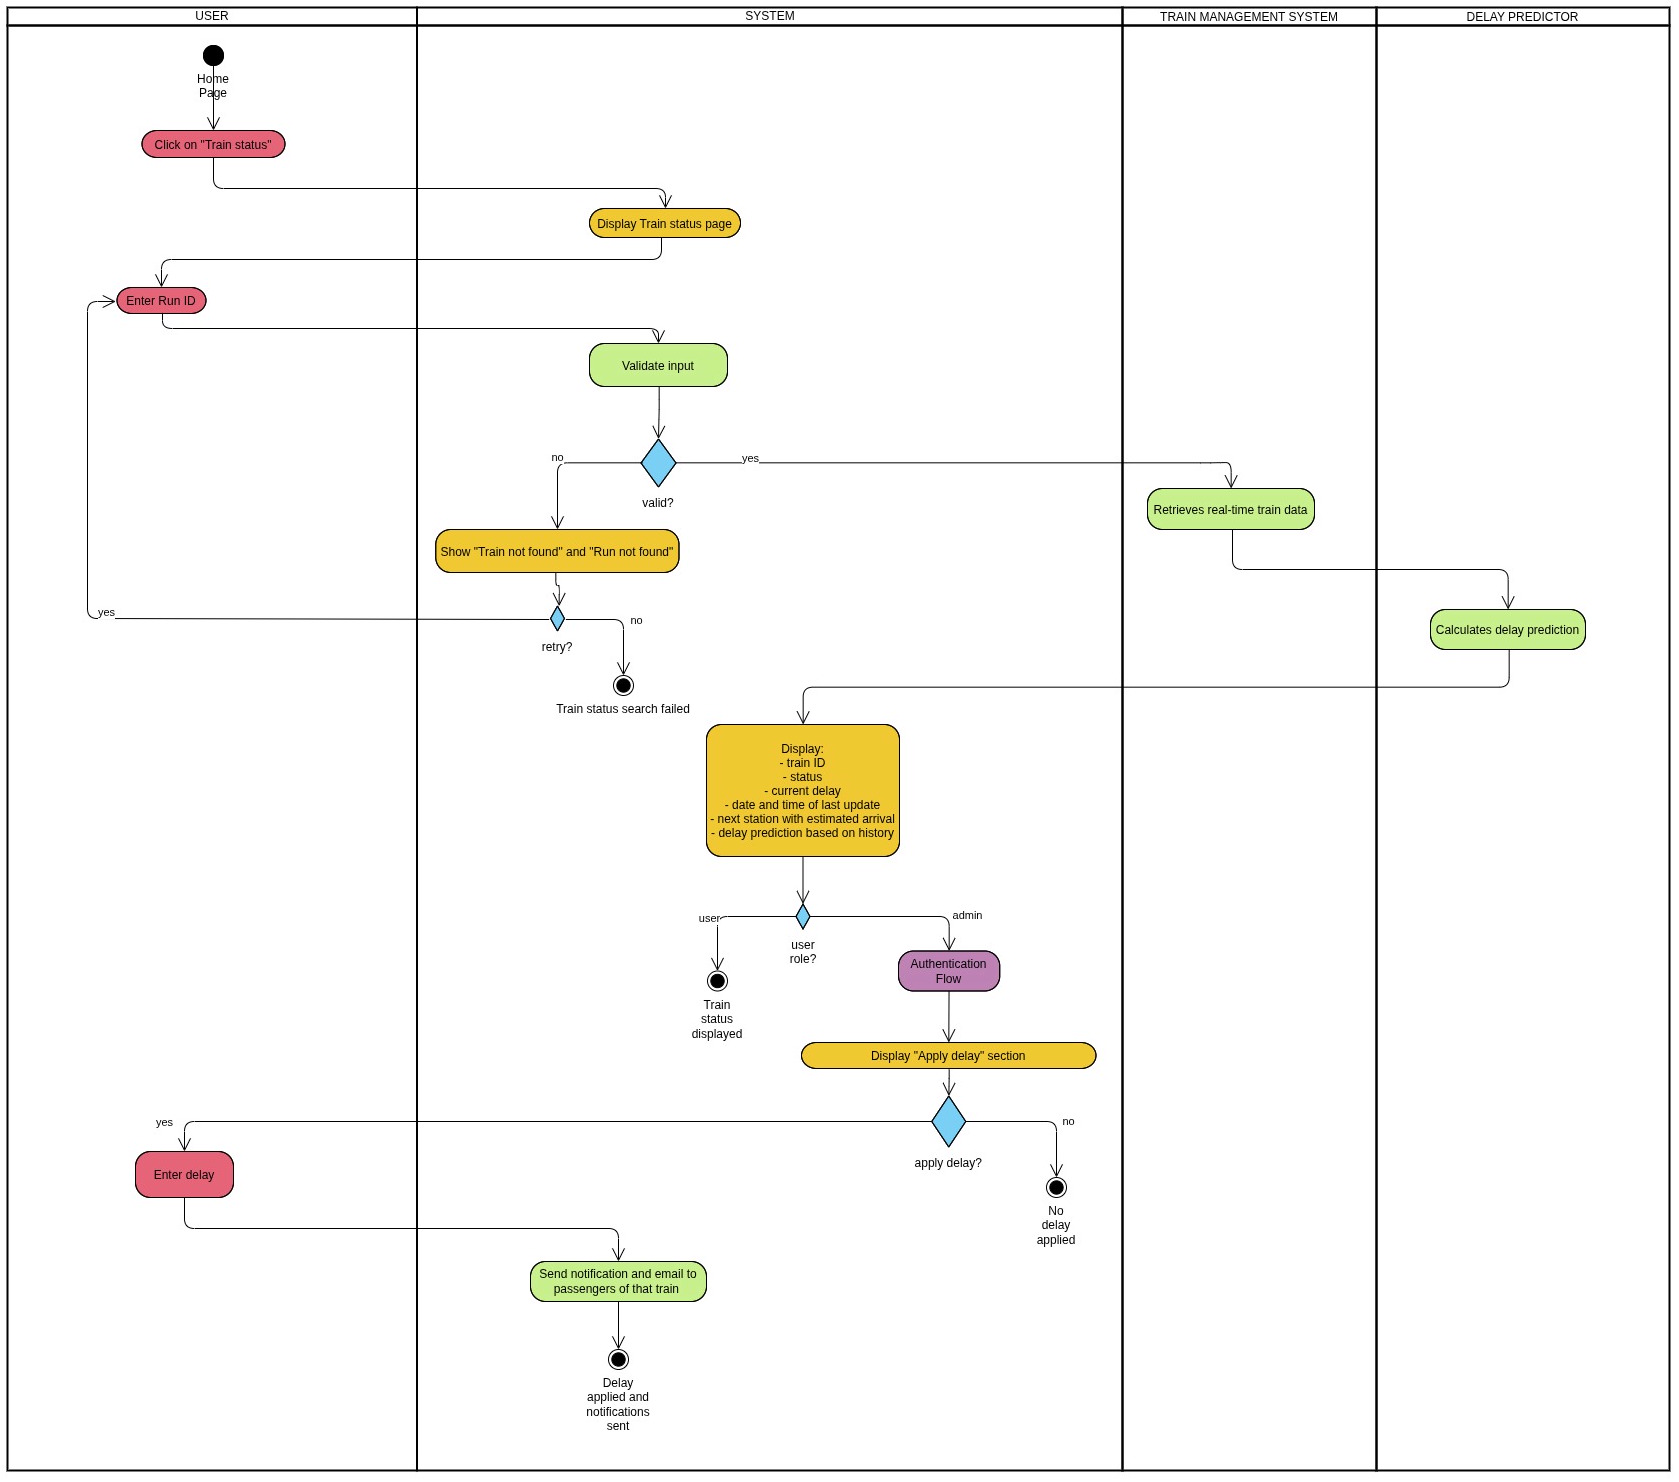
\includegraphics[width=0.9\linewidth]{Train Status and Delay Prediction Flow.jpg}
    \label{fig:placeholder}
\end{figure}
\newpage

\subsection{Customer Support Request Flow}
-Related FR: FR22
\begin{figure}[H]
    \centering
    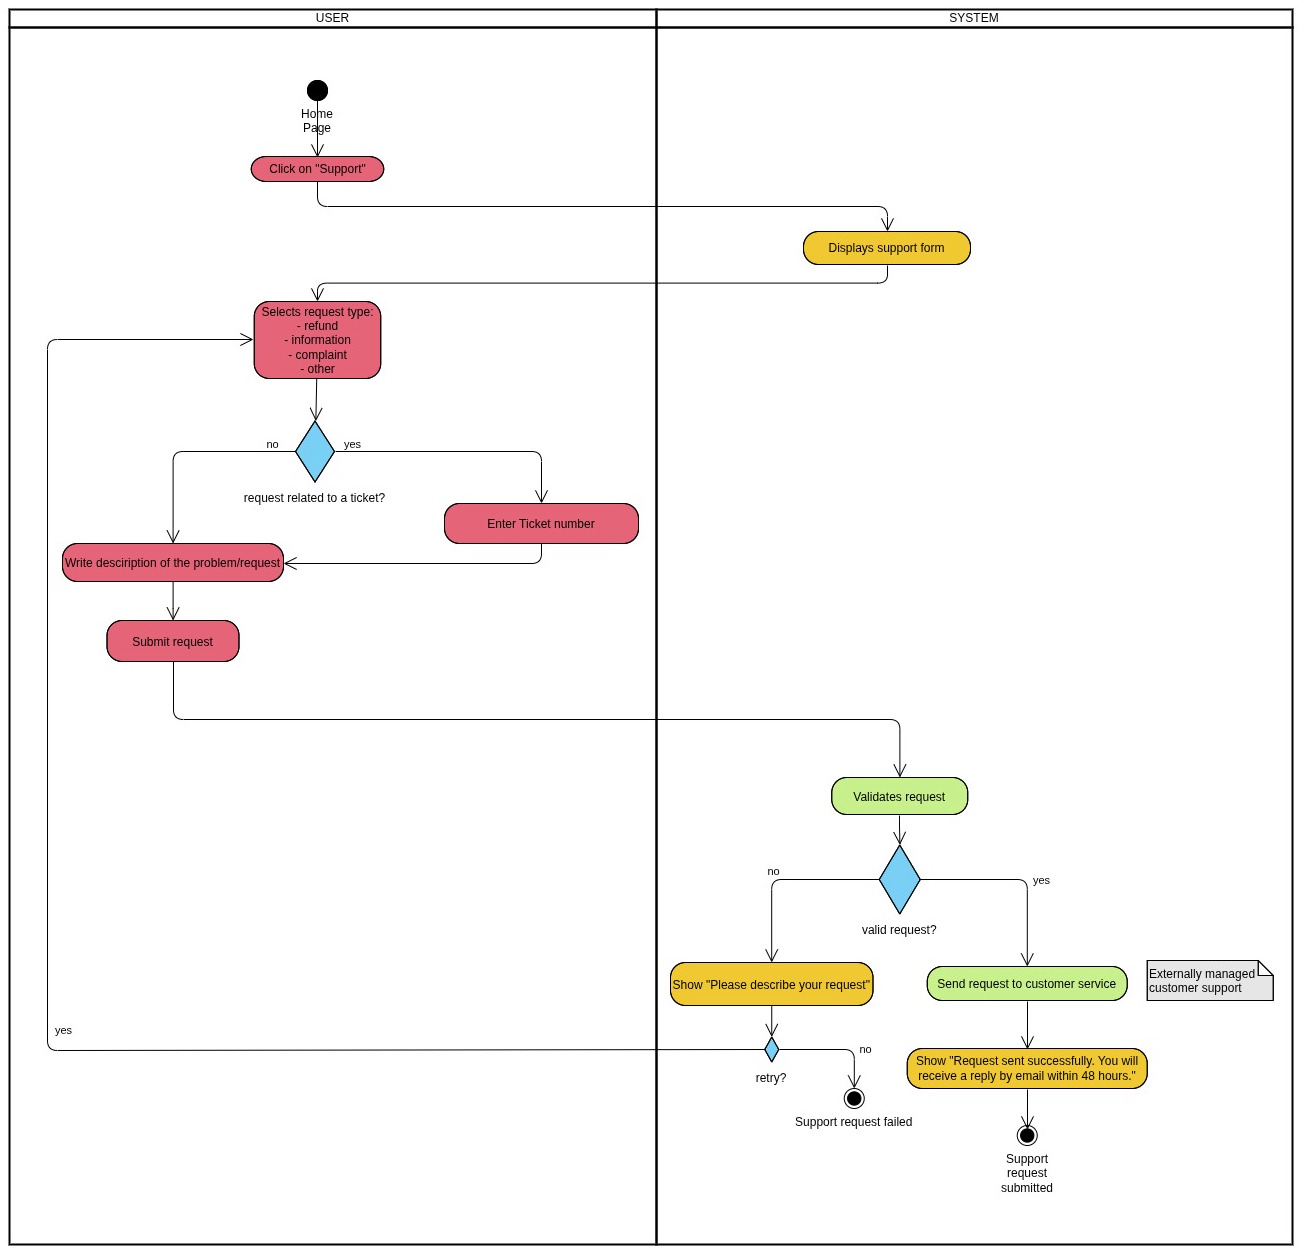
\includegraphics[width=0.9\linewidth]{Customer Support Request Flow.jpg}
    \label{fig:placeholder}
\end{figure}
\newpage

\subsection{Inspector Operations}
\label{sec:ticketvalidation}
-Related FR: FR24, FR25
\begin{figure}[H]
    \centering
    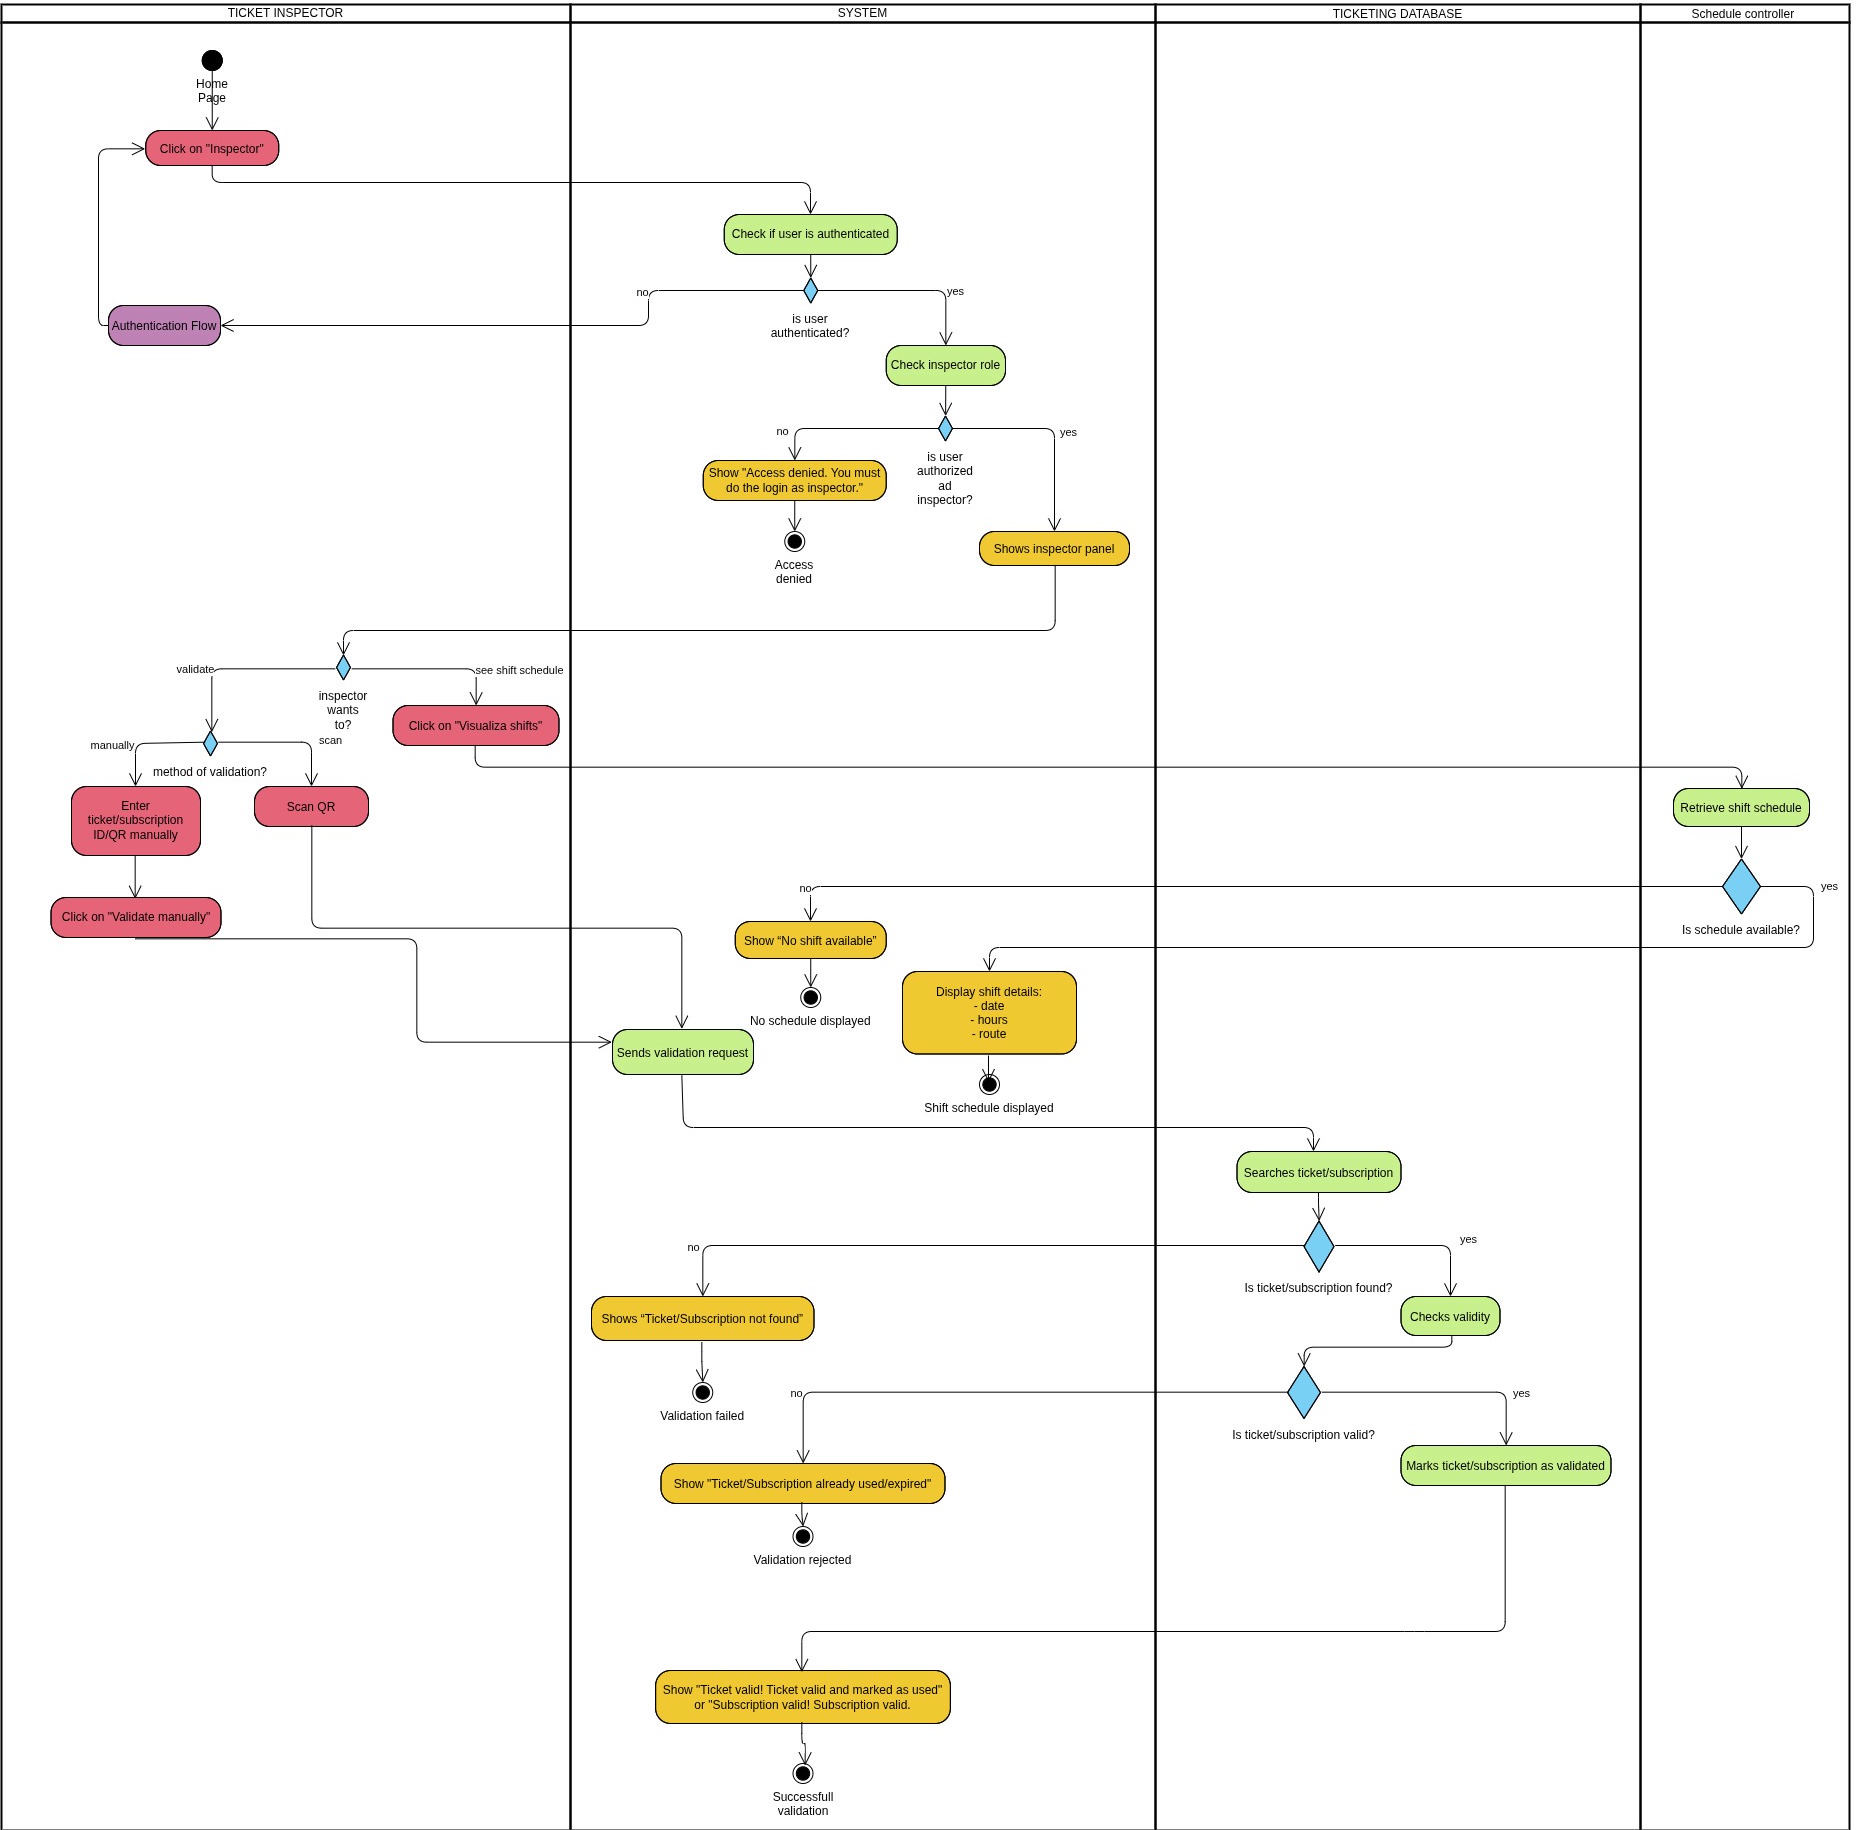
\includegraphics[width=0.9\linewidth]{Inspector Operations Flow.jpg}
    \label{fig:placeholder}
\end{figure}
\newpage

\subsection{Statistics and Insights Flow}
-Related FR: FR31, FR32
\begin{figure}[H]
    \centering
    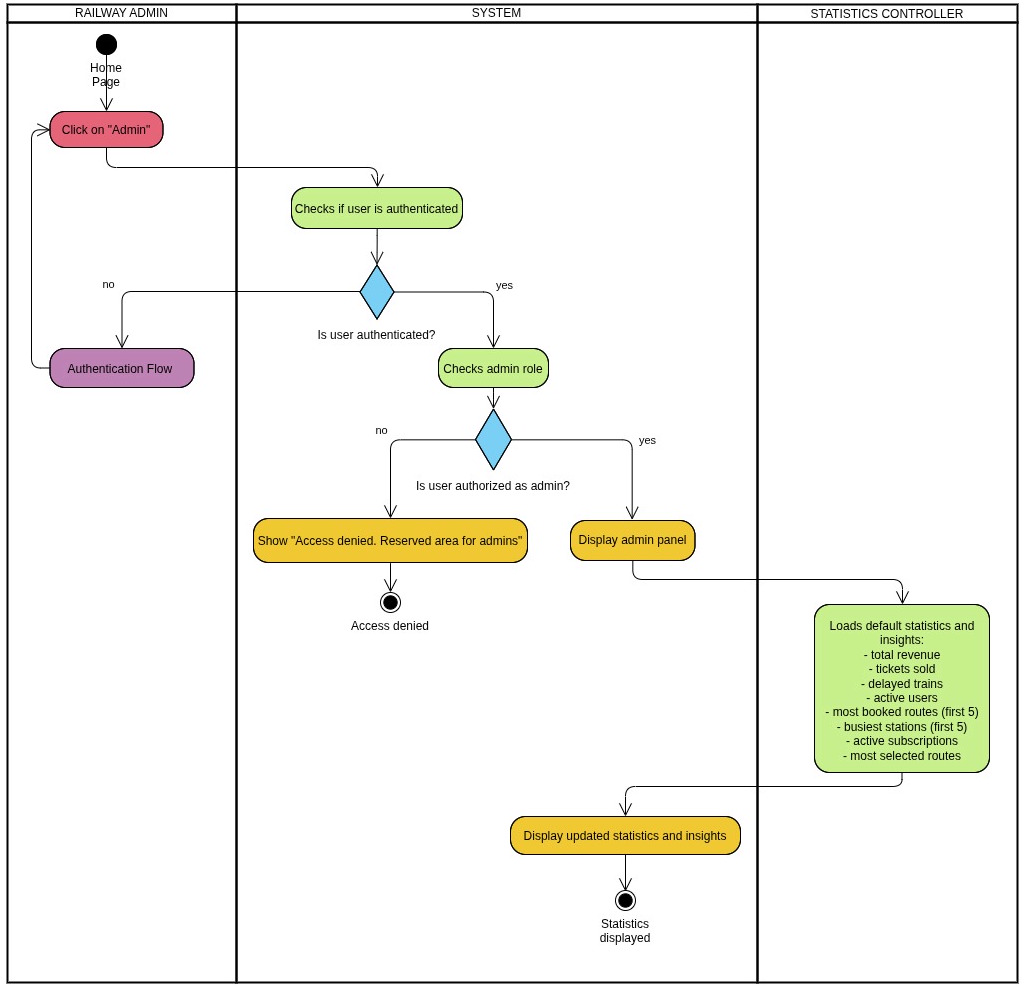
\includegraphics[width=0.9\linewidth]{Statistics and Insights Flow.jpg}
    \label{fig:placeholder}
\end{figure}
\newpage

\subsection{Notification Flow}
-Related FR: FR23
\begin{figure}[H]
    \centering
    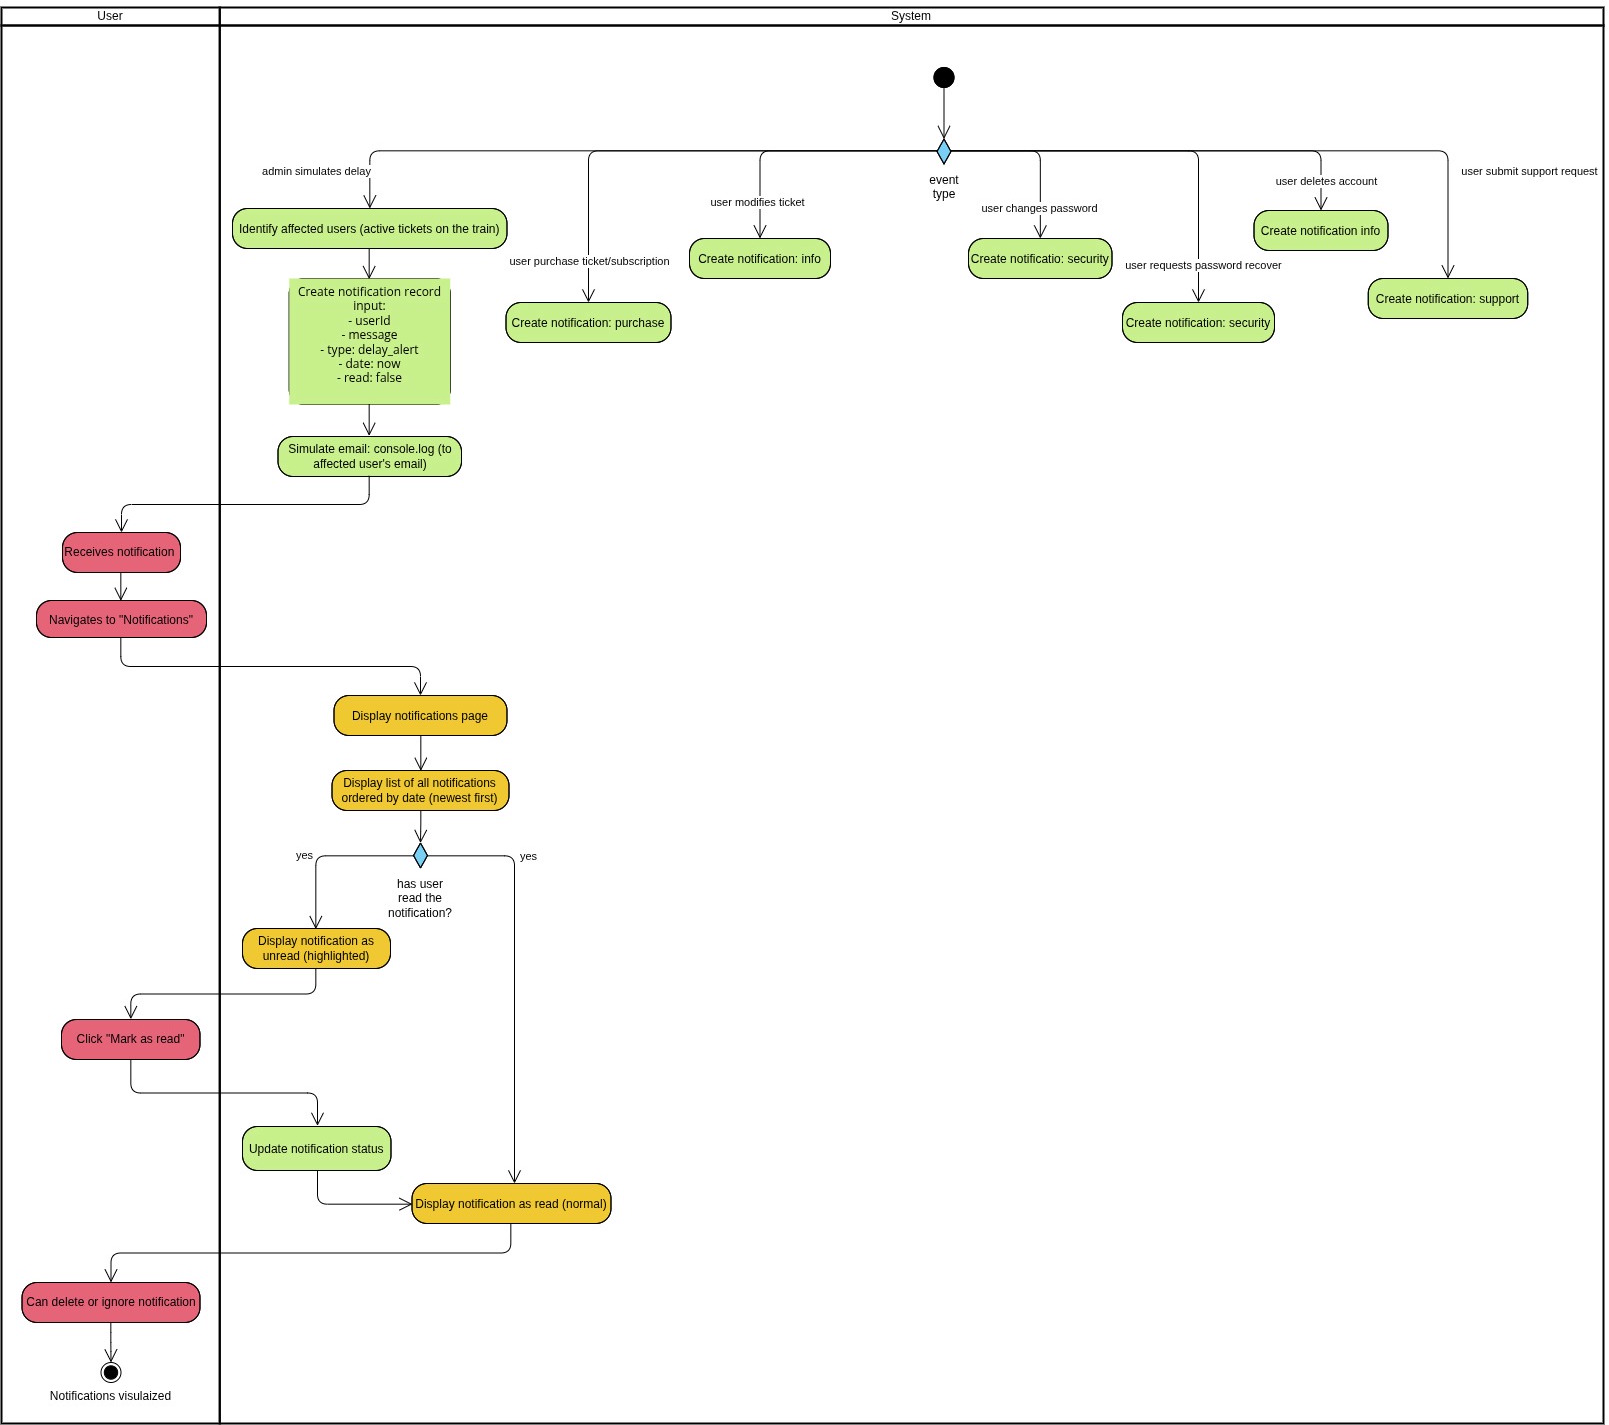
\includegraphics[width=0.9\linewidth]{Notification Flow.jpg}
    \label{fig:placeholder}
\end{figure}
\newpage

\subsection{Search Train Flow}
-Related FR: FR1, FR2, FR3, FR4, FR5, FR11
\begin{figure}[H]
    \centering
    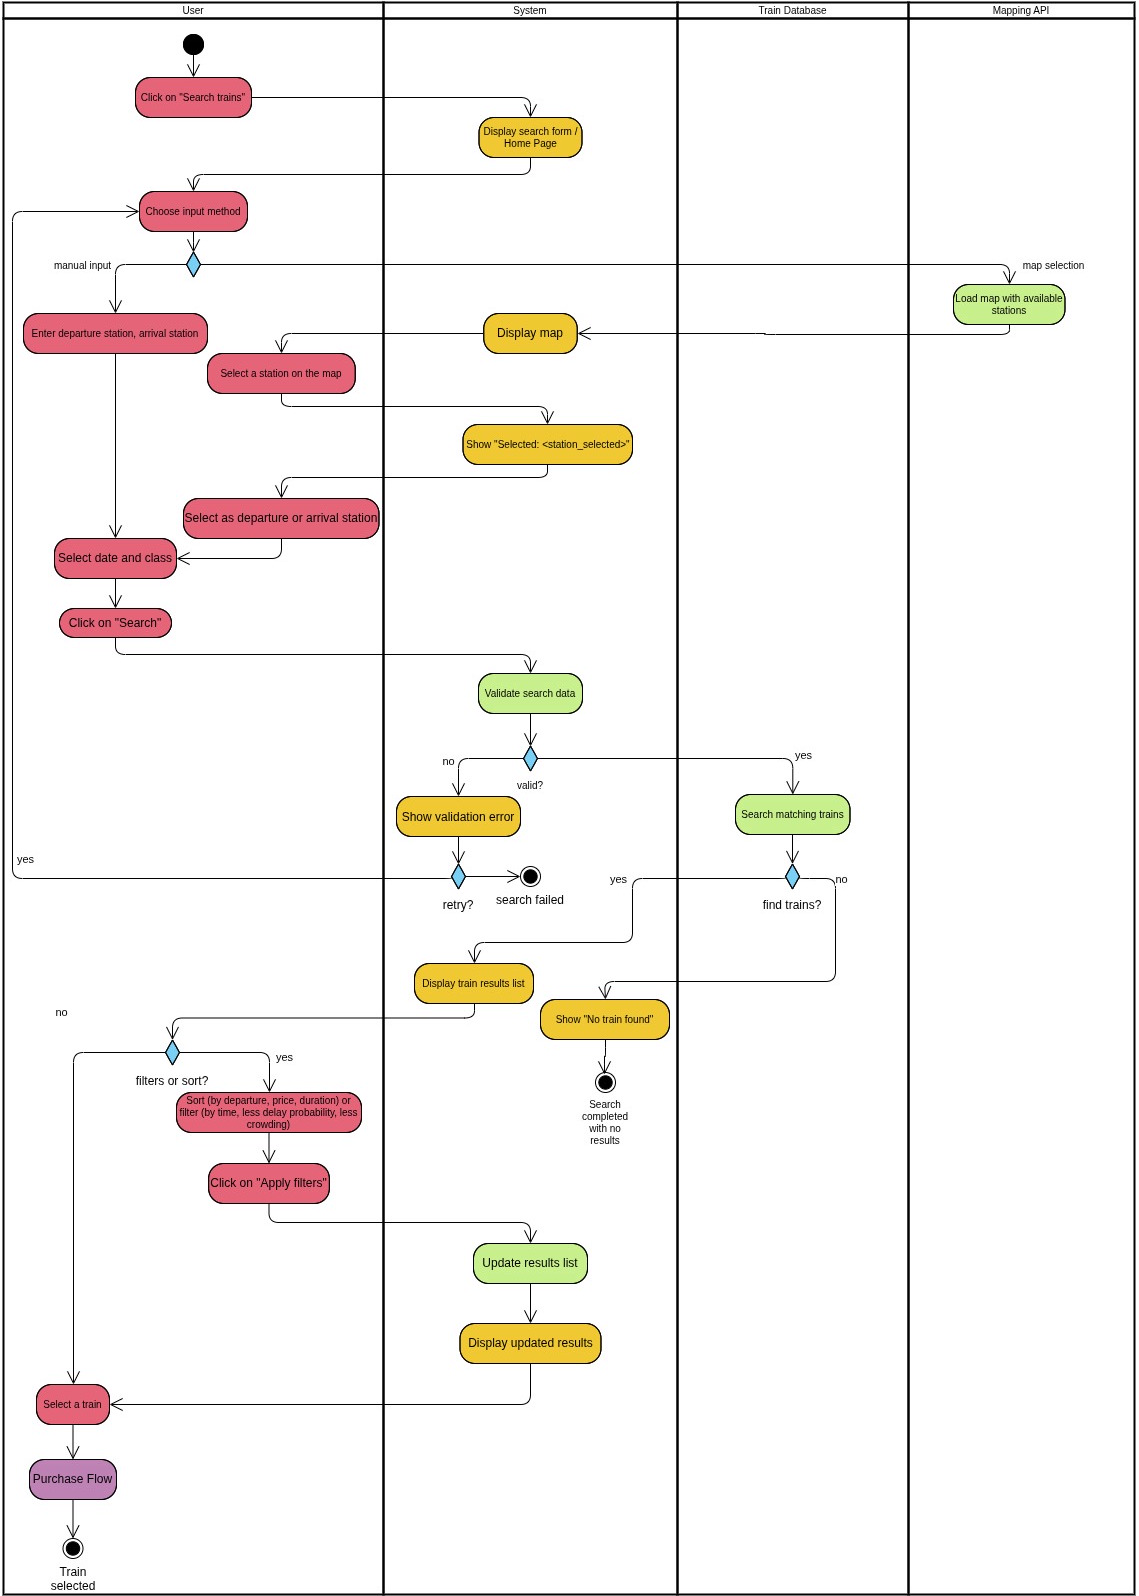
\includegraphics[width=0.9\linewidth]{Search Train Flow.jpg}
    \label{fig:placeholder}
\end{figure}
\newpage

\subsection{Ticket Purchase Flow}
-Related FR: FR8, FR9, FR10, FR13, FR19, FR21, FR26
\begin{figure}[H]
    \centering
    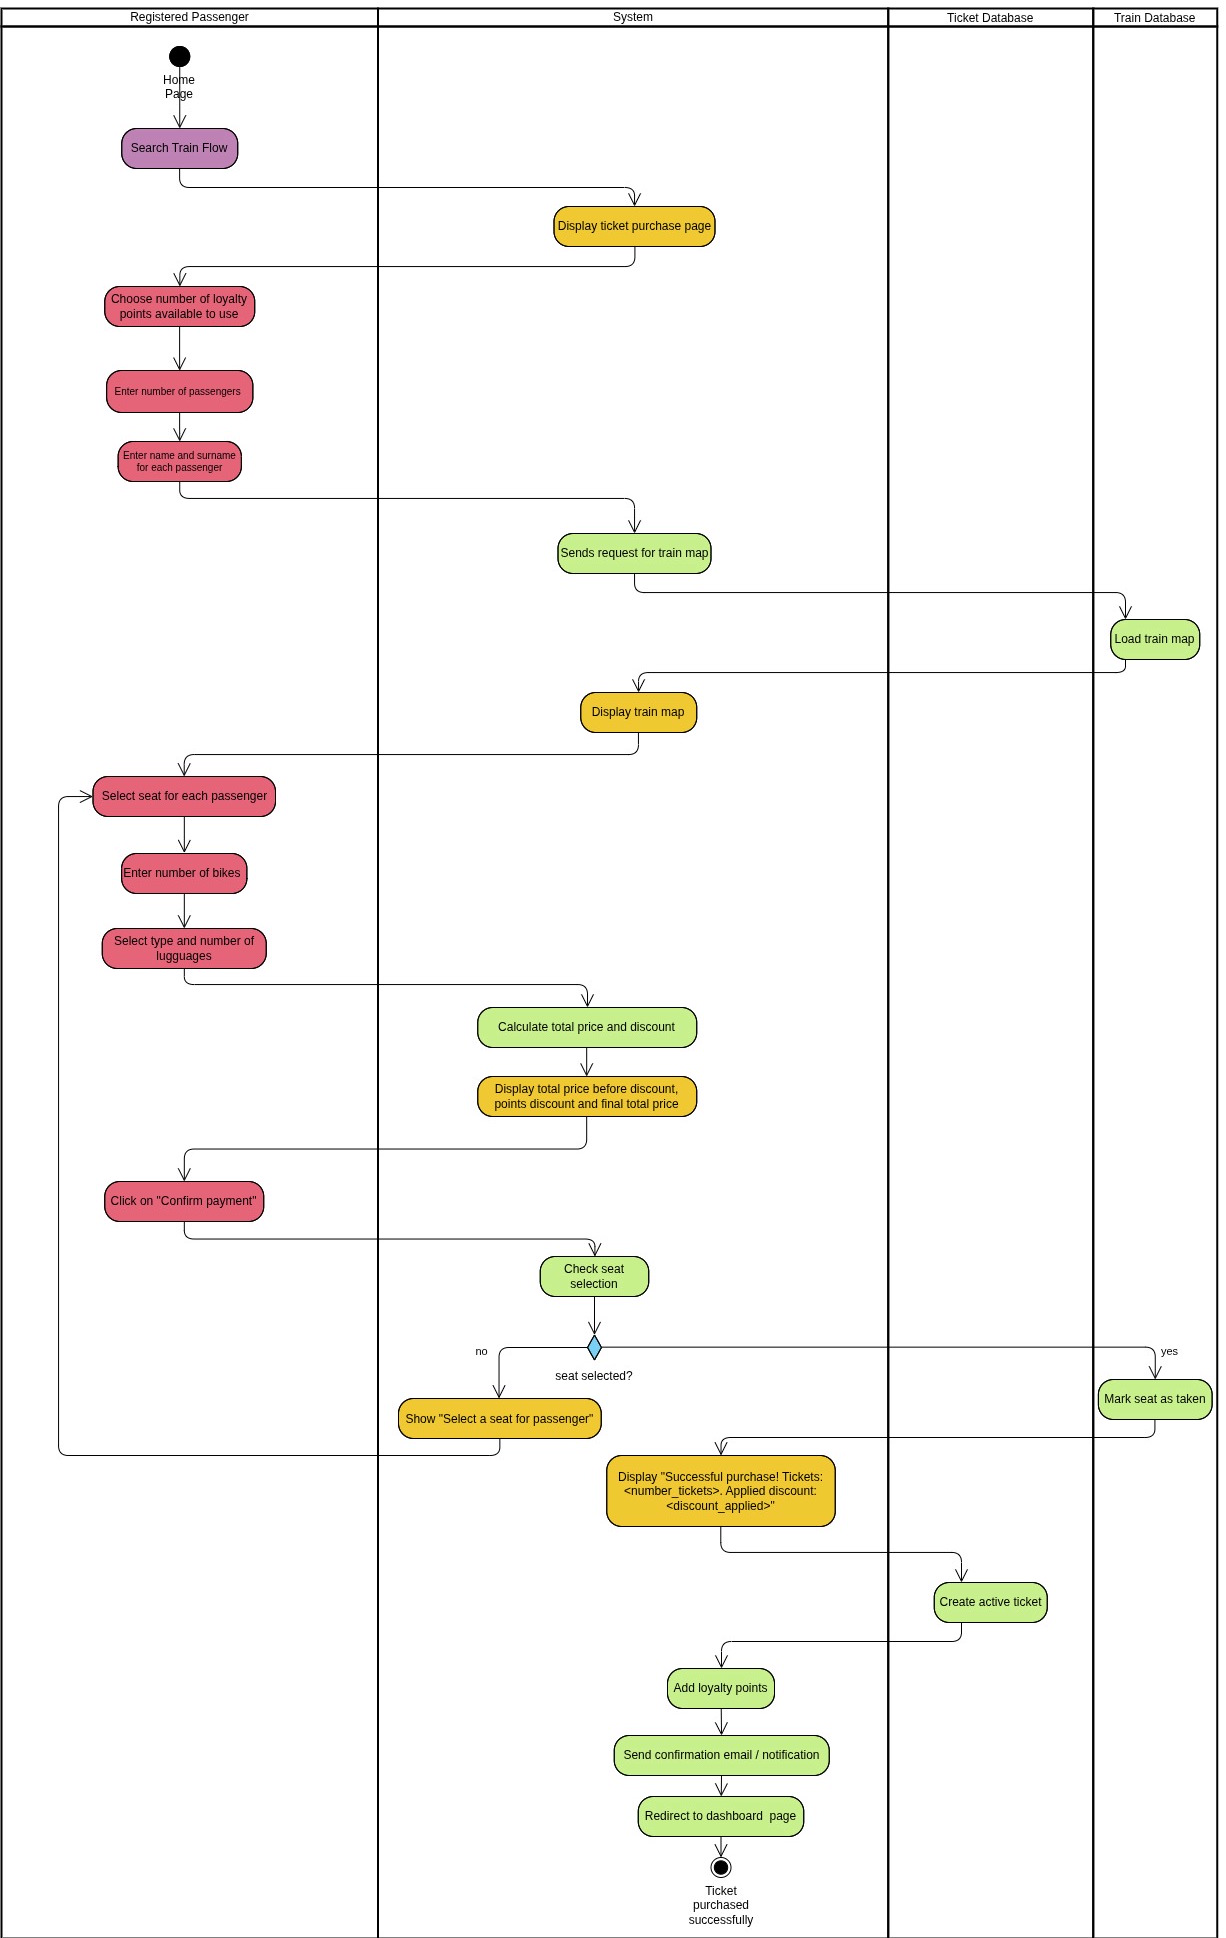
\includegraphics[width=0.8\linewidth]{Ticket Purchase Flow.jpg}
    \label{fig:placeholder}
\end{figure}
\newpage

\subsection{Subscription Purchase Flow}
-Related FR: FR14, FR19
\begin{figure}[H]
    \centering
    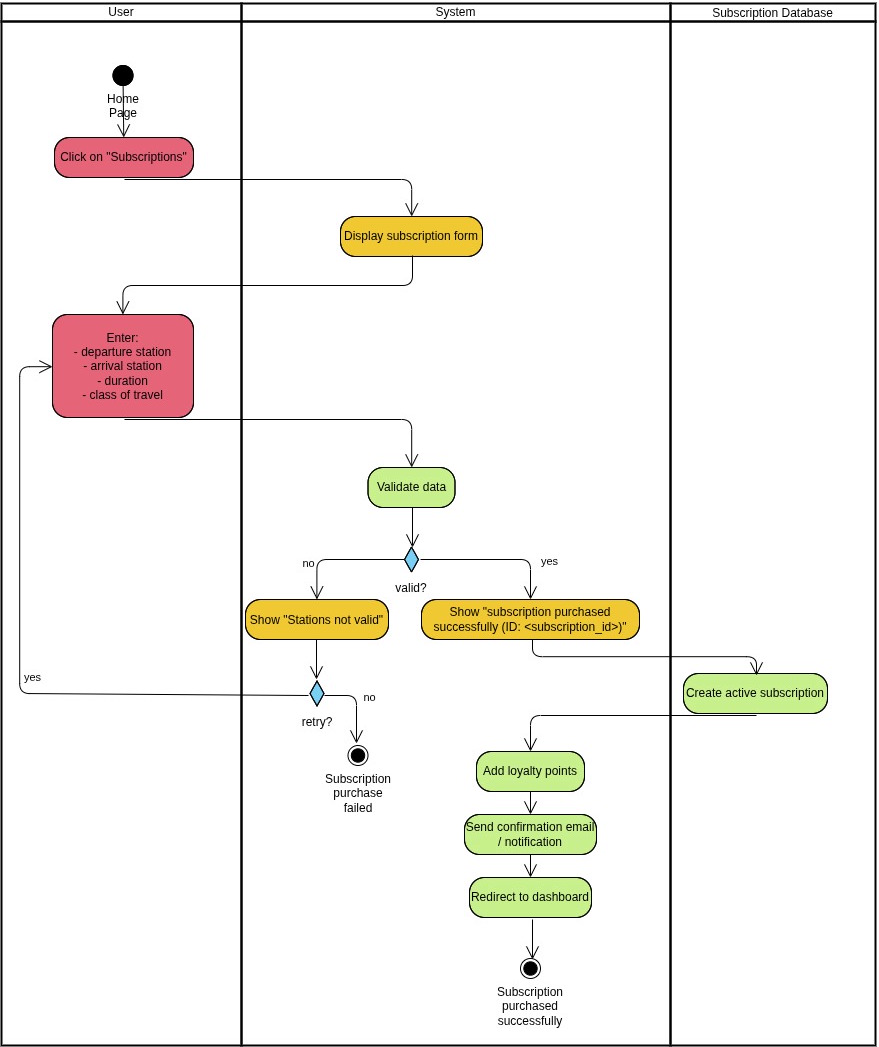
\includegraphics[width=0.9\linewidth]{Subscription Purchase Flow.jpg}
    \label{fig:placeholder}
\end{figure}
\newpage

\subsection{Payment Flow}
The payment process should have worked like this in our web app but we couldn't do it for security reasons. Also it was not one of our goals for this project. \\
-Related FR: FR13, FR14, NFR19, NFR24
\begin{figure}[H]
    \centering
    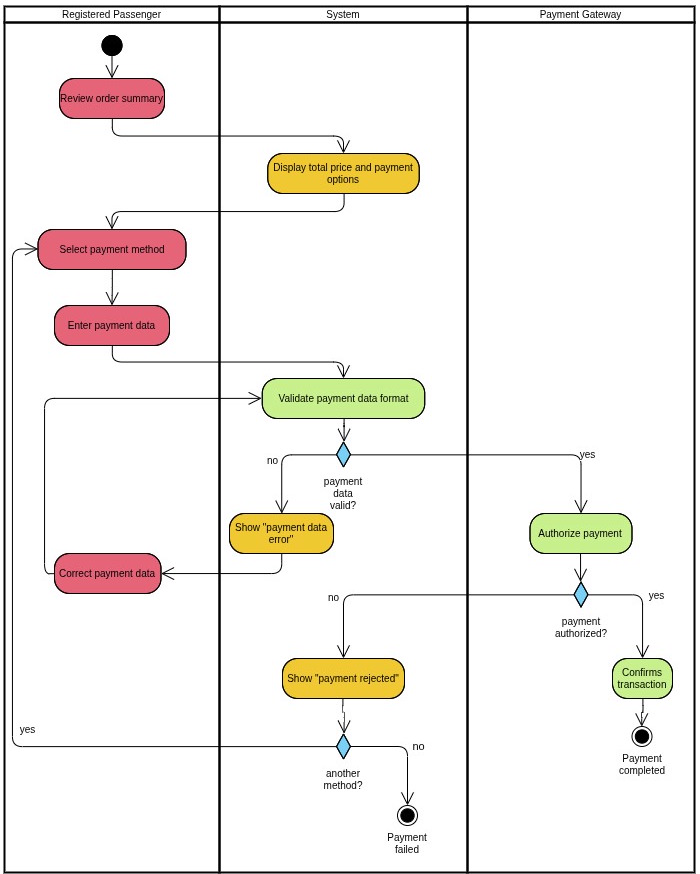
\includegraphics[width=0.9\linewidth]{Payment Flow.jpg}
    \label{fig:placeholder}
\end{figure}
\newpage

\subsection{User Dashboard Flow}
-Related FR: FR7, FR17, FR18, FR20
\begin{figure}[H]
    \centering
    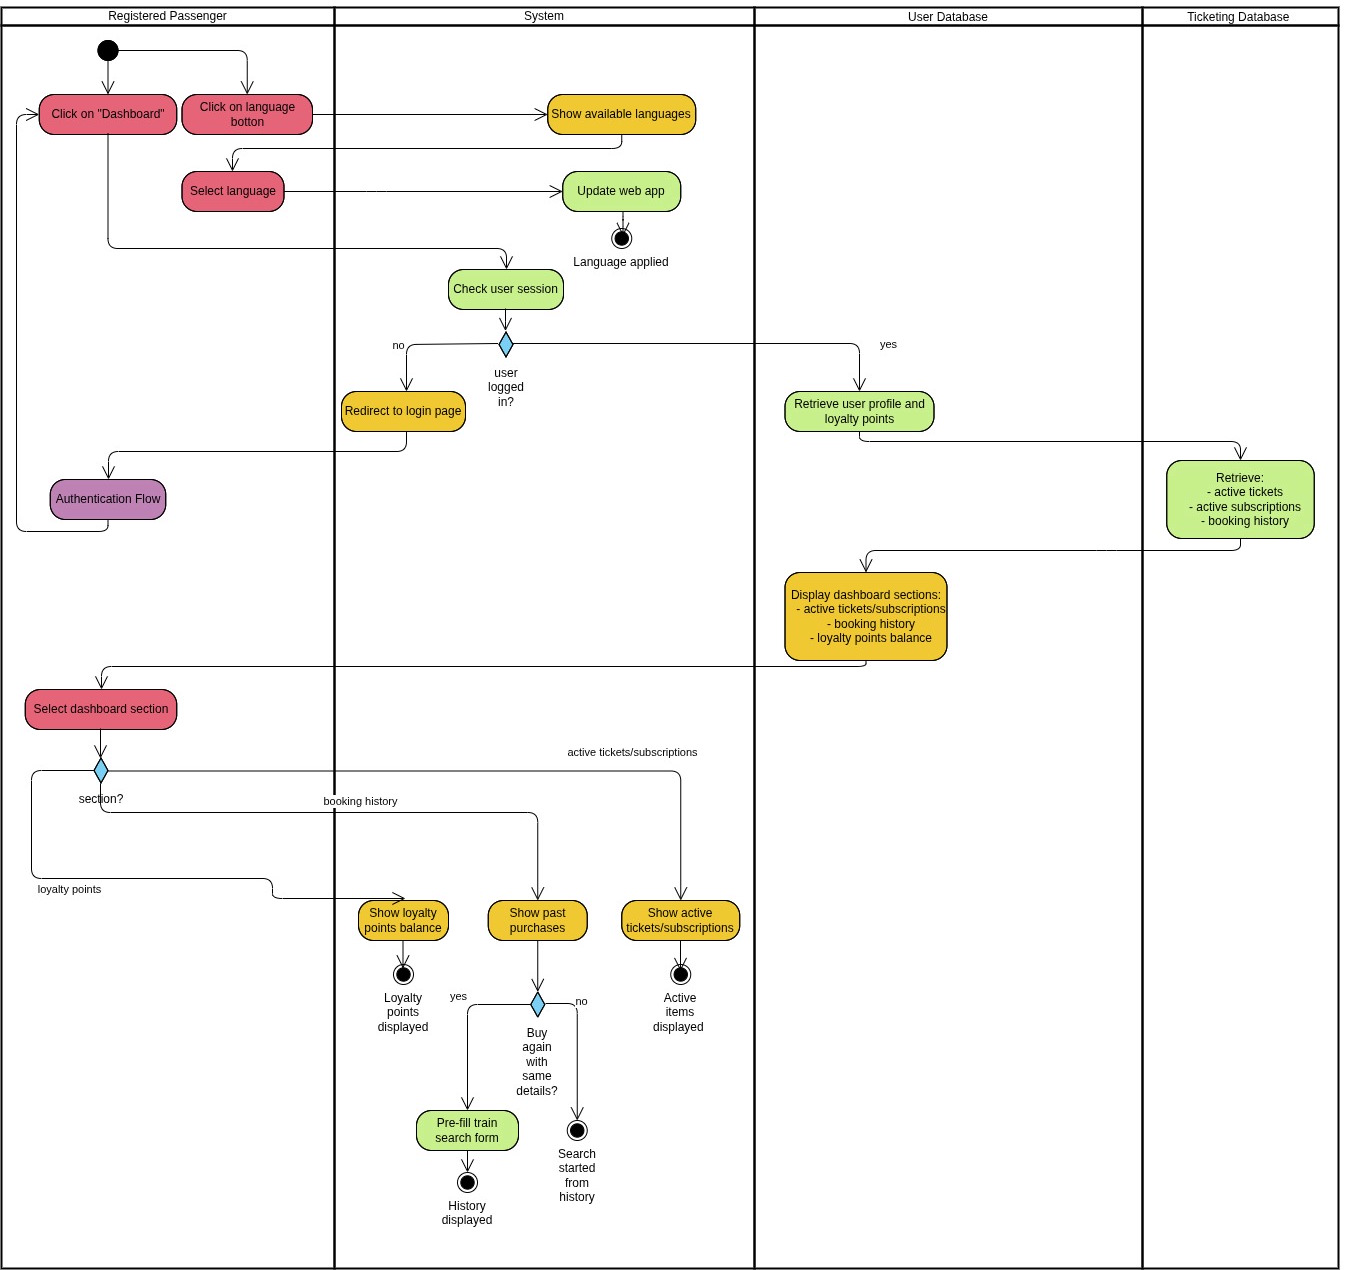
\includegraphics[width=0.9\linewidth]{User Dashboard Flow.jpg}
    \label{fig:placeholder}
\end{figure}
\newpage

\subsection{Ticket Management Flow}
-Related FR: FR16
\begin{figure}[H]
    \centering
    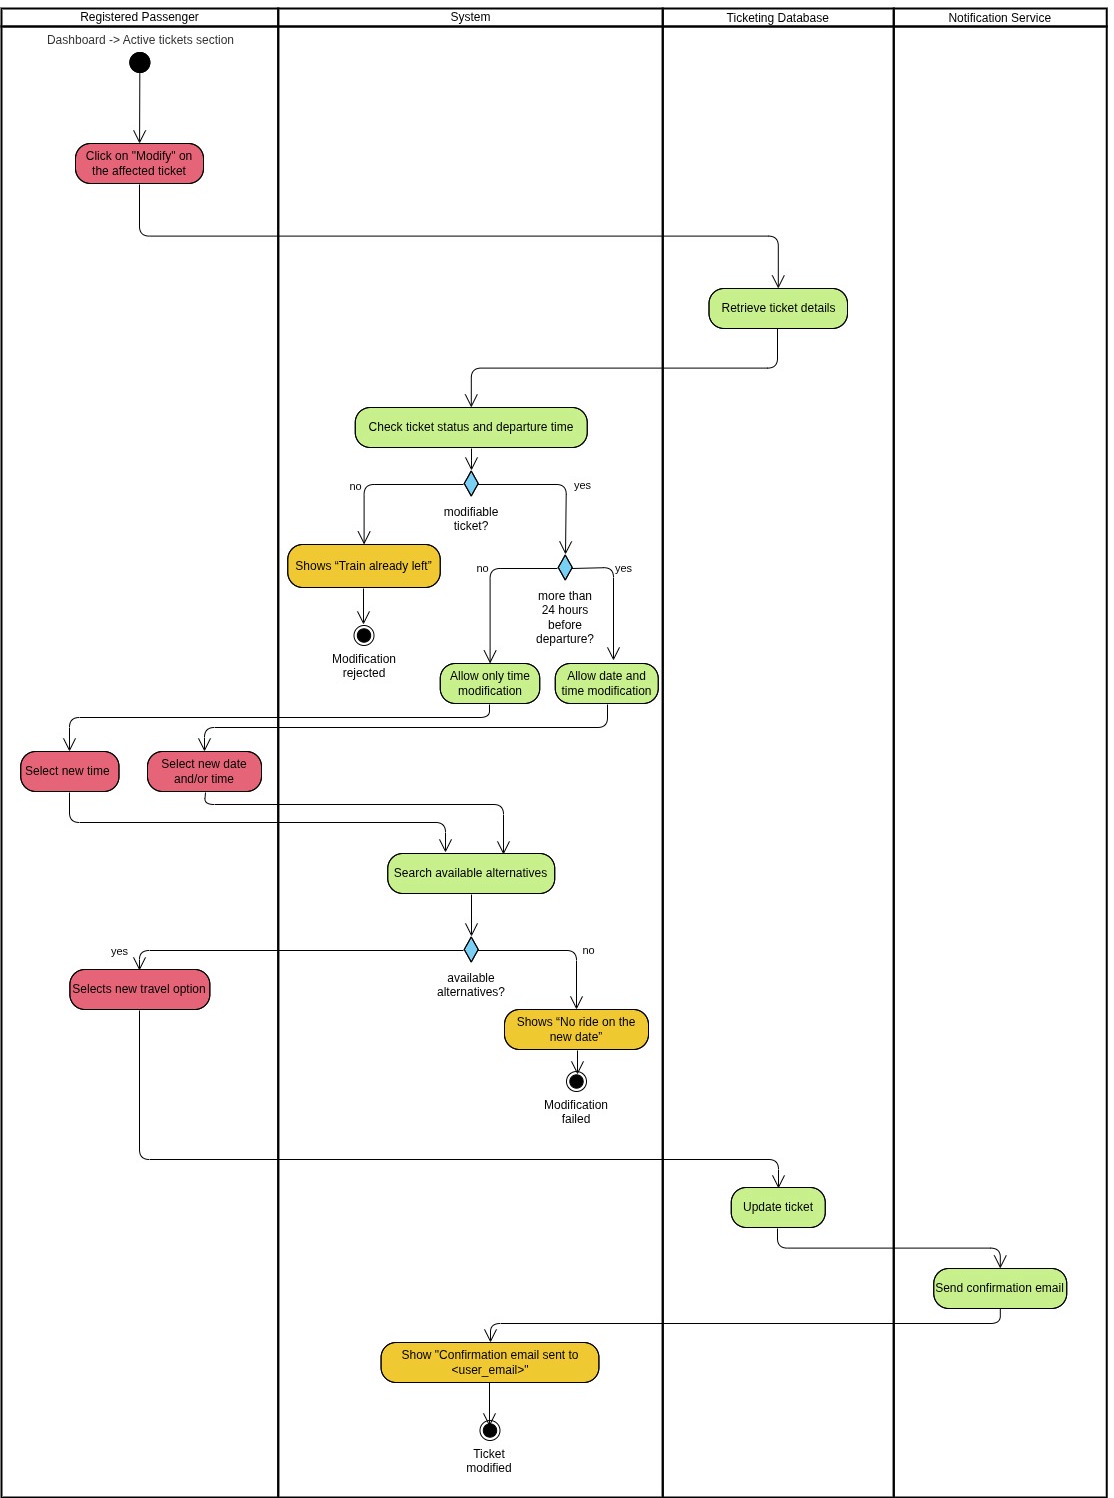
\includegraphics[width=0.8\linewidth]{Ticket Management Flow.jpg}
    \label{fig:placeholder}
\end{figure}
\newpage

\subsection{Departures Visualization Flow}
-Related FR: FR6
\begin{figure}[H]
    \centering
    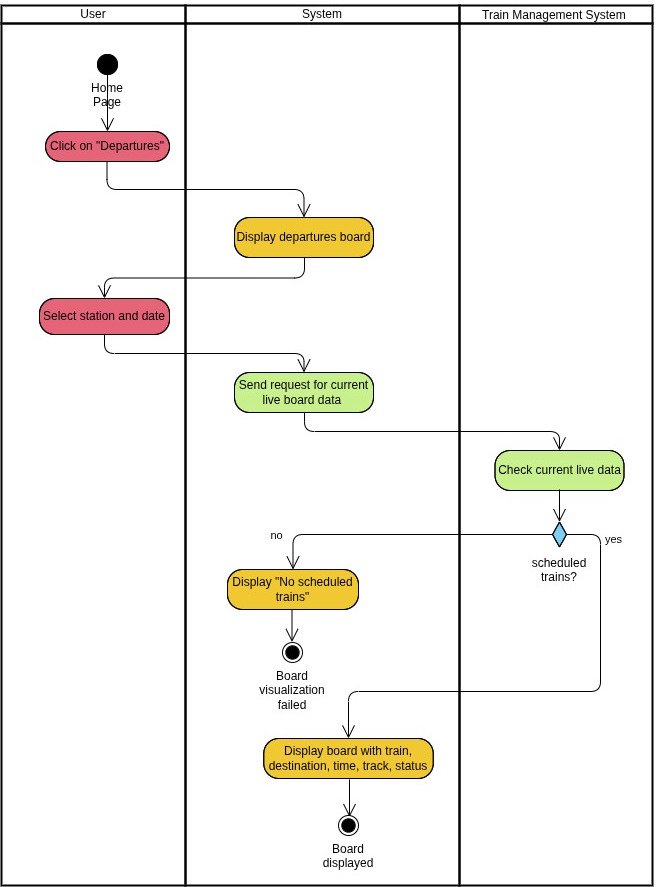
\includegraphics[width=0.8\linewidth]{Departures Visualization Flow.jpg}
    \label{fig:placeholder}
\end{figure}

\section{Code Development}
\setminted{breaklines=true}
\subsection{Project Structure}

\noindent
\begin{minipage}[t]{0.48\textwidth}
\footnotesize
\begin{verbatim}
JS Version/
├── app.js
├── package.json
├── package-lock.json
├── public/
|   ├── css/
│   │   ├── navbar.css
|   ├── js/
│   │   ├── navbar.js
│   ├── admin.html
│   ├── dashboard.html
│   ├── index.html
│   ├── inspector.html
│   ├── login.html
│   ├── notifications.html
│   ├── purchase.html
│   ├── register.html
│   ├── subscription.html
│   ├── support.html
│   ├── tabellone.html
│   ├── test-api.html
│   ├── train-status.html
│   └── images/
│       └── 104okok.png
├── src/
│   ├── controllers/
│   │   ├── AccountController.js
│   │   ├── AdminController.js
│   │   ├── ApplicationInterface.js
│   │   ├── AuthController.js
│   │   ├── InspectorController.js
│   │   ├── LanguageController.js
│   │   ├── NotificationController.js
│   │   ├── ScheduleController.js
│   │   ├── StationBoardController.js
│   │   ├── StatisticsController.js
│   │   ├── SubscriptionController.js
│   │   ├── SupportController.js
│   │   ├── TicketManagementController.js
│   │   ├── TicketPurchaseController.js
│   │   ├── TrainSearchController.js
│   │   ├── UserController.js
│   │   ├── UserDashboardController.js
│   │   └── ValidationController.js
│   ├── database/
│   │   ├── database.json
│   │   ├── db.js
│   │   ├── TicketDatabase.js
│   │   ├── TrainDatabase.js
│   │   └── UserDatabase.js
│   ├── enums/
│   │   ├── AccountStatus.js
│   │   ├── BoardEntryStatus.js
│   │   ├── BoardType.js
│   │   ├── ChangeType.js
│   │   ├── DocumentStatus.js
│   │   ├── Language.js
│   │   ├── NotificationType.js
│   │   ├── PassengerType.js
│   │   ├── PaymentStatus.js
│   │   ├── ReservationStatus.js
│   │   ├── SeatStatus.js
│   │   ├── SupportRequestStatus.js
│   │   ├── SupportRequestType.js
│   │   ├── TrainRunStatus.js
│   │   ├── TrainType.js
│   │   └── TravelClass.js
\end{verbatim}
\end{minipage}%
\hfill
\begin{minipage}[t]{0.48\textwidth}
\footnotesize
\begin{verbatim}
│   ├── externals/
│   │   ├── LoginAPI.js
│   │   ├── MappingAPI.js
│   │   └── PaymentGatewayAPI.js
│   ├── models/
│   │   ├── AdditionalReservation.js
│   │   ├── AnonymousUser.js
│   │   ├── BoardEntry.js
│   │   ├── BookingHistory.js
│   │   ├── Coach.js
│   │   ├── CustomerSupportAgent.js
│   │   ├── Dashboard.js
│   │   ├── DelayEstimate.js
│   │   ├── lang.js
│   │   ├── Notification.js
│   │   ├── OccupancyPanel.js
│   │   ├── Passenger.js
│   │   ├── PaymentDetails.js
│   │   ├── PaymentResult.js
│   │   ├── PaymentTransaction.js
│   │   ├── PredictionSystem.js
│   │   ├── RailwayAdministrator.js
│   │   ├── RegisteredUser.js
│   │   ├── Route.js
│   │   ├── SearchCriteria.js
│   │   ├── Seat.js
│   │   ├── SessionToken.js
│   │   ├── Station.js
│   │   ├── StationBoard.js
│   │   ├── StatisticsFilter.js
│   │   ├── StatisticsReport.js
│   │   ├── Stop.js
│   │   ├── Subscription.js
│   │   ├── SupportRequest.js
│   │   ├── Ticket.js
│   │   ├── TicketChangeRequest.js
│   │   ├── TicketInspector.js
│   │   ├── Train.js
│   │   ├── TrainOption.js
│   │   ├── TrainRun.js
│   │   ├── TrainSearchResult.js
│   │   ├── TrainStatus.js
│   │   ├── TravelDocument.js
│   │   ├── TravelDocumentSummary.js
│   │   ├── User.js
│   │   ├── UserProfile.js
│   │   ├── ValidationPanel.js
│   │   └── ValidationResult.js
│   └── utils/
│       ├── crypto.js
│       ├── geo.js
│       ├── Location.js
│       ├── notifications.js
│       ├── PaymentDetails.js
│       ├── PaymentResult.js
│       ├── SearchCriteria.js
│       ├── SessionToken.js
│       ├── StatisticsFilter.js
│       ├── TicketChangeRequest.js
│       └── ValidationResult.js
└── node_modules/
    └── ... (dependencies omitted for brevity)
\end{verbatim}
\end{minipage}

\subsection{API Development}
This section lists all REST API endpoints implemented in the web application.
Each entry includes classification (Internal / Simulated), description,
related Use Cases, and the corresponding route definition from \texttt{app.js}.
% ----------------------------------------------------------------------
\subsubsection*{API 1: GET /api/stations}
\textbf{Classification:} Internal (station data from internal database).\\
\textbf{Description:} Returns the list of all railway stations with their identifiers,
coordinates and codes. Used for search forms and maps.\\
\textbf{Related Use Cases:} UC1 (Search Train), UC6 (Boards Visualization).
\begin{minted}[frame=lines,linenos]{javascript}
app.get('/api/stations', (req, res) => {
    res.json(getStations());
});
\end{minted}

% ----------------------------------------------------------------------
\subsubsection*{API 2: POST /api/language}
\textbf{Classification:} Internal (user language preference management).\\
\textbf{Description:} Allows an authenticated user to change the interface language.
The preference is stored in the user profile and persists across sessions.\\
\textbf{Related Use Cases:} UC15 (Change Language).
\begin{minted}[frame=lines,linenos]{javascript}
app.post('/api/language', AuthController.setLanguage);
\end{minted}

% ----------------------------------------------------------------------
\subsubsection*{API 3: POST /api/login}
\textbf{Classification:} Simulated (should be external – Login API, NFR24).\\
\textbf{Description:} Authenticates a user. According to NFR24 this should be delegated
to an external OAuth2 / Login API. The current implementation verifies credentials
against the internal database, enforces failed attempt limits and session creation.\\
\textbf{Related Use Cases:} UC2 (Authentication).
\begin{minted}[frame=lines,linenos]{javascript}
app.post('/api/login', AuthController.login);
\end{minted}

% ----------------------------------------------------------------------
\subsubsection*{API 4: POST /api/register}
\textbf{Classification:} Simulated (should be external – Login API, NFR24).\\
\textbf{Description:} Registers a new user. Email uniqueness and password strength
are checked. According to requirements this should be handled by an external
identity provider.\\
\textbf{Related Use Cases:} UC2 (Authentication).
\begin{minted}[frame=lines,linenos]{javascript}
app.post('/api/register', AuthController.register);
\end{minted}

% ----------------------------------------------------------------------
\subsubsection*{API 5: POST /api/search}
\textbf{Classification:} Internal (train search based on internal database and prediction system).\\
\textbf{Description:} Searches for direct trains between two stations on a specific date.
Applies filters (travel class, train type) and calculates price, delay probability,
crowding probability using the internal delay prediction module (OB2).\\
\textbf{Related Use Cases:} UC1 (Search Train), UC5 (Check Train Status).
\begin{minted}[frame=lines,linenos]{javascript}
app.post('/api/search', TrainSearchController.search);
\end{minted}

% ----------------------------------------------------------------------
\subsubsection*{API 6: POST /api/search-advanced}
\textbf{Classification:} Internal (search with transfers).\\
\textbf{Description:} Extends the basic search to allow up to one train change.
Computes waiting times and combines segments into a single itinerary.\\
\textbf{Related Use Cases:} UC1 (Search Train).
\begin{minted}[frame=lines,linenos]{javascript}
app.post('/api/search-advanced', TrainSearchController.searchAdvanced);
\end{minted}

% ----------------------------------------------------------------------
\subsubsection*{API 7: GET /api/train-status/:runId}
\textbf{Classification:} Internal (real‑time status from Train Management System).\\
\textbf{Description:} Provides current location (next station) and delay information
for a specific train run. Data is taken from the internal train runs database.\\
\textbf{Related Use Cases:} UC5 (Check Train Status).
\begin{minted}[frame=lines,linenos]{javascript}
app.get('/api/train-status/:runId', TrainSearchController.getTrainStatus);
\end{minted}

% ----------------------------------------------------------------------
\subsubsection*{API 8: GET /api/predict-delay/:runId}
\textbf{Classification:} Internal (delay prediction module – OB2).\\
\textbf{Description:} Returns a delay prediction for a given train run based on
historical delay data. The prediction module is internal as per OB2.\\
\textbf{Related Use Cases:} UC1 (Search Train), UC5 (Check Train Status).
\begin{minted}[frame=lines,linenos]{javascript}
app.get('/api/predict-delay/:runId', TrainSearchController.predictDelay);
\end{minted}

% ----------------------------------------------------------------------
\subsubsection*{API 9: GET /api/departures/:stationId}
\textbf{Classification:} Internal (real‑time departure board – FR6).\\
\textbf{Description:} Returns the list of upcoming departures from a given station
on a specified date, including scheduled times, tracks and delay status.\\
\textbf{Related Use Cases:} UC6 (Boards Visualization).
\begin{minted}[frame=lines,linenos]{javascript}
app.get('/api/departures/:stationId', StationBoardController.getDepartures);
\end{minted}

% ----------------------------------------------------------------------
\subsubsection*{API 10: POST /api/recover-password}
\textbf{Classification:} Simulated (should be external – Login API, NFR24).\\
\textbf{Description:} Initiates password recovery by sending a reset email
(simulated). According to NFR24 this should be delegated to an external service.\\
\textbf{Related Use Cases:} UC10 (Account Management).
\begin{minted}[frame=lines,linenos]{javascript}
app.post('/api/recover-password', AuthController.recoverPassword);
\end{minted}

% ----------------------------------------------------------------------
\subsubsection*{API 11: GET /api/me}
\textbf{Classification:} Internal (current user data).\\
\textbf{Description:} Returns basic information (id, name, role) of the
authenticated user. Requires a valid session token.\\
\textbf{Related Use Cases:} UC2 (Authentication), UC8 (User Dashboard/Profile).
\begin{minted}[frame=lines,linenos]{javascript}
app.get('/api/me', UserController.getMe);
\end{minted}

% ----------------------------------------------------------------------
\subsubsection*{API 12: GET /api/user/dashboard/:userId}
\textbf{Classification:} Internal (user dashboard).\\
\textbf{Description:} Retrieves active tickets, purchase history, and loyalty
points for a specific user. Access is restricted to the user themselves or an
administrator.\\
\textbf{Related Use Cases:} UC8 (User Dashboard/Profile), UC9 (Ticket Management).
\begin{minted}[frame=lines,linenos]{javascript}
app.get('/api/user/dashboard/:userId', UserController.getDashboard);
\end{minted}

% ----------------------------------------------------------------------
\subsubsection*{API 13: GET /api/user/points}
\textbf{Classification:} Internal (loyalty points).\\
\textbf{Description:} Returns the loyalty points balance of the authenticated user.
Points are earned per euro spent (NFR29).\\
\textbf{Related Use Cases:} UC8 (User Dashboard/Profile).
\begin{minted}[frame=lines,linenos]{javascript}
app.get('/api/user/points', UserController.getPoints);
\end{minted}

% ----------------------------------------------------------------------
\subsubsection*{API 14: GET /api/seat-map/:runId}
\textbf{Classification:} Internal (seat map for selection).\\
\textbf{Description:} Returns the seat configuration (free/occupied) for a
specific train run, used during ticket purchase to allow seat selection (FR8).\\
\textbf{Related Use Cases:} UC4 (Purchase).
\begin{minted}[frame=lines,linenos]{javascript}
app.get('/api/seat-map/:runId', TicketPurchaseController.getSeatMap);
\end{minted}

% ----------------------------------------------------------------------
\subsubsection*{API 15: POST /api/purchase}
\textbf{Classification:} Simulated (should use external Payment Gateway API – NFR19).\\
\textbf{Description:} Processes the purchase of a ticket including seat selection,
extra services (bike, luggage) and loyalty points discount. Payment is simulated
internally; a real implementation would call Stripe/PayPal.\\
\textbf{Related Use Cases:} UC4 (Purchase).
\begin{minted}[frame=lines,linenos]{javascript}
app.post('/api/purchase', TicketPurchaseController.purchase);
\end{minted}

% ----------------------------------------------------------------------
\subsubsection*{API 16: PUT /api/ticket}
\textbf{Classification:} Internal (ticket modification – FR16).\\
\textbf{Description:} Modifies date and/or time of an already purchased ticket,
respecting the 24‑hour policy (full change if >24h, time only if ≤24h).\\
\textbf{Related Use Cases:} UC9 (Ticket Management).
\begin{minted}[frame=lines,linenos]{javascript}
app.put('/api/ticket', UserController.modifyTicket);
\end{minted}

% ----------------------------------------------------------------------
\subsubsection*{API 17: POST /api/change-password}
\textbf{Classification:} Simulated (should be external – Login API, NFR24).\\
\textbf{Description:} Changes the password of the authenticated user after
verifying the old password. According to NFR24 this should be delegated.\\
\textbf{Related Use Cases:} UC10 (Account Management).
\begin{minted}[frame=lines,linenos]{javascript}
app.post('/api/change-password', UserController.changePassword);
\end{minted}

% ----------------------------------------------------------------------
\subsubsection*{API 18: POST /api/logout}
\textbf{Classification:} Internal (session management).\\
\textbf{Description:} Terminates the user session by deleting the server-side
session token.\\
\textbf{Related Use Cases:} UC2 (Authentication).
\begin{minted}[frame=lines,linenos]{javascript}
app.post('/api/logout', UserController.logout);
\end{minted}

% ----------------------------------------------------------------------
\subsubsection*{API 19: DELETE /api/account}
\textbf{Classification:} Internal (account deletion – FR27, GDPR).\\
\textbf{Description:} Permanently deletes the user account and all associated
personal data, after checking that no active tickets exist. Implements the
“right to be forgotten”.\\
\textbf{Related Use Cases:} UC10 (Account Management).
\begin{minted}[frame=lines,linenos]{javascript}
app.delete('/api/account', UserController.deleteAccount);
\end{minted}

% ----------------------------------------------------------------------
\subsubsection*{API 20: POST /api/validate}
\textbf{Classification:} Internal (ticket validation – FR24, OB6).\\
\textbf{Description:} Allows a ticket inspector (role `inspector`) to validate
a passenger's ticket, marking it as used and updating coach occupancy.\\
\textbf{Related Use Cases:} UC12 (Inspector Operations Management).
\begin{minted}[frame=lines,linenos]{javascript}
app.post('/api/validate', InspectorController.validateTicket);
\end{minted}

% ----------------------------------------------------------------------
\subsubsection*{API 21: GET /api/inspector/schedule/:inspectorId}
\textbf{Classification:} Internal (shift schedule – FR25, OB8).\\
\textbf{Description:} Returns the shift calendar for an authenticated inspector,
including dates, start/end times, assigned route and train code.\\
\textbf{Related Use Cases:} UC13 (Shift Schedule Visualization).
\begin{minted}[frame=lines,linenos]{javascript}
app.get('/api/inspector/schedule/:inspectorId', InspectorController.getSchedule);
\end{minted}

% ----------------------------------------------------------------------
\subsubsection*{API 22: GET /api/admin/stats}
\textbf{Classification:} Internal (statistics for administrators – OB9, FR32).\\
\textbf{Description:} Provides aggregate metrics (revenue, total bookings,
delayed trains, active users, top routes, top stations) for administrative staff.\\
\textbf{Related Use Cases:} UC14 (Statistics Visualization), UC3 (Admin Area Access).
\begin{minted}[frame=lines,linenos]{javascript}
app.get('/api/admin/stats', AdminController.getStats);
\end{minted}

% ----------------------------------------------------------------------
\subsubsection*{API 23: POST /api/support}
\textbf{Classification:} Internal (customer support – FR22, OB7).\\
\textbf{Description:} Registers a support request (refund, information, report)
from a user. Stores the request with status `open` for customer service.\\
\textbf{Related Use Cases:} UC11 (Customer Support).
\begin{minted}[frame=lines,linenos]{javascript}
app.post('/api/support', SupportController.submit);
\end{minted}

% ----------------------------------------------------------------------
\subsubsection*{API 24: GET /api/notifications}
\textbf{Classification:} Internal (user notifications – FR23).\\
\textbf{Description:} Returns the list of notifications for the authenticated user
(e.g., delay alerts, purchase confirmations, password changes).\\
\textbf{Related Use Cases:} UC7 (Receive Notifications), UC8 (User Dashboard/Profile).
\begin{minted}[frame=lines,linenos]{javascript}
app.get('/api/notifications', NotificationController.getNotifications);
\end{minted}

% ----------------------------------------------------------------------
\subsubsection*{API 25: PUT /api/notifications/:id/read}
\textbf{Classification:} Internal (notification management).\\
\textbf{Description:} Marks a specific notification as read.\\
\textbf{Related Use Cases:} UC7 (Receive Notifications).
\begin{minted}[frame=lines,linenos]{javascript}
app.put('/api/notifications/:id/read', NotificationController.markAsRead);
\end{minted}

% ----------------------------------------------------------------------
\subsubsection*{API 26: POST /api/subscription}
\textbf{Classification:} Simulated (should use external Payment Gateway – NFR19).\\
\textbf{Description:} Purchases a subscription (regional or single‑route).
Calculates price based on distance and duration, awards loyalty points,
and simulates payment.\\
\textbf{Related Use Cases:} UC4 (Purchase).
\begin{minted}[frame=lines,linenos]{javascript}
app.post('/api/subscription', SubscriptionController.purchase);
\end{minted}

% ----------------------------------------------------------------------
\subsubsection*{API 27: GET /api/routes}
\textbf{Classification:} Internal (route data for subscription).\\
\textbf{Description:} Returns the list of available routes (origin–destination pairs)
that can be subscribed to.\\
\textbf{Related Use Cases:} UC1 (Search Train), UC4 (Purchase).
\begin{minted}[frame=lines,linenos]{javascript}
app.get('/api/routes', SubscriptionController.getRoutes);
\end{minted}

% ----------------------------------------------------------------------
\subsubsection*{API 28: GET /api/subscription-price}
\textbf{Classification:} Internal (price calculation).\\
\textbf{Description:} Calculates the price of a subscription based on stations,
duration and travel class without executing a purchase.\\
\textbf{Related Use Cases:} UC4 (Purchase).
\begin{minted}[frame=lines,linenos]{javascript}
app.get('/api/subscription-price', SubscriptionController.getPrice);
\end{minted}

% ----------------------------------------------------------------------
\subsubsection*{API 29: GET /api/debug}
\textbf{Classification:} Internal (development only).\\
\textbf{Description:} Debug endpoint returning the number of stations in the
database and the number of active sessions. Not intended for production.\\
\textbf{Related Use Cases:} None (development aid).
\begin{minted}[frame=lines,linenos]{javascript}
app.get('/api/debug', (req, res) => {
    const db = readDB();
    res.json({ stationsCount: db.stations.length, sessionsCount: AuthController.sessionCount() });
});
\end{minted}

% ----------------------------------------------------------------------
\subsubsection*{API 30: POST /api/simulate-delay}
\textbf{Classification:} Internal (administrator delay simulation).\\
\textbf{Description:} Allows an administrator to simulate a delay on a train run.
Automatically generates in‑app and email notifications for all affected passengers
(implements OB2 and FR23).\\
\textbf{Related Use Cases:} UC7 (Receive Notifications), UC3 (Admin Area Access).
\begin{minted}[frame=lines,linenos]{javascript}
app.post('/api/simulate-delay', AdminController.simulateDelay);
\end{minted}

\section{GitHub Repository}
\label{sec:cta_code}

\begin{center}
    \setlength{\fboxsep}{15pt} % Spessore del pulsante (padding interno)
    \href{https://github.com/tegoli/software-engineering-TRAIN}{%
        \colorbox{black}{%
            \parbox{0.65\textwidth}{%
                \centering
                \textcolor{white}{\sffamily\bfseries\large SEE IT IN ACTION $\downarrow$}\\
                \vspace{5pt}
                \textcolor{gray}{\sffamily\scriptsize EXPLORE THE FULL REPOSITORY ON GITHUB}
                \textbf{CLICK HERE}
            }%
        }%
    }
\end{center}

% ============================================================================
% SECTION: TEAM ROLES
% ============================================================================
\section{Team Assessment}

\subsection{Work Organization}
From the start of the project we decided to split the work equally, we made sure to be aligned on the desire to follow the schedule of the project. The task were split following this rules:
\begin{itemize}
    \item Equal division of the workload
    \item Affinity for a specific task
\end{itemize}
Maintaining the criteria mentioned above, permitted us to fully understand each topic, since everyone tried to do everything.


\subsection{Roles and Activities}
\begin{table}[htbp]
\centering
\small
% Distribuiamo i pesi delle colonne X: la seconda (D2) ha più testo, quindi le diamo più spazio economico
\begin{tabularx}{\textwidth}{@{} >{\bfseries}l >{\hsize=0.8\hsize}X >{\hsize=1.4\hsize}X >{\hsize=0.8\hsize}X @{}}
\toprule
 & \multicolumn{3}{c}{\textbf{Main Contributions}} \\
\cmidrule(l){2-4}
\textbf{Team Member} & \textbf{Deliverable 1 (D1)} & \textbf{Deliverable 2 (D2)} & \textbf{Deliverable 3 (D3)} \\
\midrule
MATTEO   & Non-Functional \newline Requirements & 
  \textbf{Assigned Use Cases:} \newline
  UC12, UC13, UC14, UC15 \newline
  \addlinespace[2pt]
  \textit{For each of the above:} \newline
  • Use Case Specification \newline
  • Sequence Diagram \newline
  • Activity Diagram \newline
   \textbf{Additional Artifacts:} \newline
  • LaTeX formatting \newline \textit{(with all diagrams and tables)}  \newline  
  • Use Case Diagram \newline
  & • Database \& Implementation  \newline
  • Front-End Development \newline
  • Documentation \\
\addlinespace
ROBIN    & Objectives                  & 
  \textbf{Assigned Use Cases:} \newline
  UC1, UC2, UC3 \newline
  \addlinespace[2pt]
  \textit{For each of the above:} \newline
  • Use Case Specification \newline
  • Sequence Diagram \newline
  • Activity Diagram \newline
  \addlinespace[4pt]
  \textbf{Additional Artifacts:} \newline
  • State Diagram & 
  • API Implementation \newline
  • Documentation \newline
  • Skeleton and Structure of Project \newline
  • Front-End Development\\
\addlinespace
VIRGINIA & Stakeholders                & 
  \textbf{Assigned Use Cases:} \newline
  UC4, UC5, UC6, UC7 \newline
  \addlinespace[2pt]
  \textit{For each of the above:} \newline
  • Use Case Specification \newline
  • Sequence Diagram \newline
  • Activity Diagram & •  User-Flow \newline • Testing\\
\addlinespace
CATERINA & Functional \newline Requirements     & 
  \textbf{Assigned Use Cases:} \newline
  UC8, UC9, UC10, UC11 \newline
  \addlinespace[2pt]
  \textit{For each of the above:} \newline
  • Use Case Specification \newline
  • Sequence Diagram \newline
  • Activity Diagram & • User-Flow\newline • Testing \\
\midrule
\textbf{Shared Artifacts} & \multicolumn{3}{p{\dimexpr\textwidth-15\tabcolsep}@{}}{%
\textbf{Global Class Diagram:} Developed collaboratively by all team members as a single, unified system architecture model.%
} \\
\addlinespace
\textbf{All Members} & \multicolumn{3}{p{\dimexpr\textwidth-15\tabcolsep}@{}}{%
\textbf{Cross-Review and Quality Assurance:} For each Deliverable (D1, D2, D3), a comprehensive peer-review process was conducted by all team members to ensure global consistency, alignment, and error correction.%
} \\
\bottomrule
\end{tabularx}
\end{table}

\subsection{Workload and Distribution}
Below is the workload expressed in percentage per deliverable for each member of the group.

\begin{table}[htbp]
\centering
\small
\begin{tabular}{@{} L{0.35\textwidth} C{0.12\textwidth} C{0.12\textwidth} C{0.12\textwidth} C{0.12\textwidth} @{}}
\toprule
 & \textbf{MATTEO} & \textbf{ROBIN} & \textbf{VIRGINIA} & \textbf{CATERINA} \\
\midrule
\textbf{D1} & 25\% & 25\% & 25\% & 25\% \\
\textbf{D2} & 25\% & 25\% & 25\% & 25\% \\
\textbf{D3} & 25\% & 25\% & 25\% & 25\% \\
\midrule
\textbf{Proposed grade} \textit{(optional)} & 30 & 30 & 30 & 30 \\
\bottomrule
\end{tabular}
\end{table}
\textbf{MOTIVATION:} To ensure equitable resource allocation, the overall workload was distributed evenly (25\% per member) throughout the software lifecycle. 
\par To mitigate communication costs and streamline development, we adopted a modular team structure composed of two sub-teams: (Robin \& Matteo) and (Caterina \& Virginia). \par This approach allowed us to capitalize on co-located workspaces (like the Acquario room for Virginia and Caterina) and synchronized schedules (as for Robin and Matteo attending in presence the same courses), significantly reducing coordination overhead during key development phases.
\par Final verification followed a strict collaborative inspection model. A mandatory review involving the entire four-member team was executed before delivery, guaranteeing system integration, maintaining conceptual integrity, and preventing architectural discrepancies.
\par From the total hours described in the table, we can see that for the first deliverable, the work was performed equally by all three members by splitting the deliverable task in 4 (OBJECTIVE, STAKEHOLDERS, FUNCTIONAL REQUIREMENT, NON-FUNCTIONAL REQUIREMENTS). 
\par For the second and third deliverable we decided on an approach in which every member did a bit of every task: for example in D2 every member took care of 4 UC designing for each and every diagram (ACTIVITY, SEQUENCE, USE CASE DESCRIPTION), while for the class diagram each developed the same number of class. 


\subsection{Critical Issues}

\par Throughout the project lifecycle and previous deliverables, it was anticipated that the Ticket Inspector would update seat occupancy after ticket validation. However, the current implementation only supports seat selection at the time of ticket purchase, meaning that season tickets (subscriptions) are currently not tracked.

Due to technical complexities and project time constraints, the complete automated tracking system by the Ticket Inspector has been deferred to future releases. Consequently, this feature has been excluded from the D3 scope, including both the user flows and the codebase implementation.

\end{document}